\documentclass[aspectratio=169, 15pt,usenames,dvipsnames]{beamer}


\usepackage[utf8]{inputenc}
\usepackage{fontspec}
\usepackage{sansmathfonts}
\usepackage{xcolor}
\usepackage{fontenc}
\usepackage{unicode-math}
\usepackage{listings}
\usepackage{cprotect}

\usepackage[makeroom]{cancel}

\usefonttheme{serif}
\usefonttheme{professionalfonts}


\usepackage[sfdefault,scaled=1.1]{FiraSans}
\usepackage{sourcecodepro}
\usepackage{graphicx}

\graphicspath{
    {themes/gd/images/},
    {images/}
}
\usepackage{themes/gd/beamerthemegd}
\usepackage{themes/gd/beamerinnerthemegd}
\usepackage{themes/gd/beamerouterthemegd}
\usepackage{themes/gd/beamercolorthemegd}


\graphicspath{
    {themes/gd/images/},
    {images/}
}

\setlength{\parskip}{1em}
\setbeamertemplate{footline}{%
   \raisebox{5pt}{\makebox[\paperwidth]{\hfill\makebox[10pt]{\scriptsize\insertframenumber}}}}

\title{Time In Distributed Systems\\Pt.1}
% \date[ISPN ’80]{27th International Symposium of Prime Numbers}
\author[Euclid]{Euclid of Alexandria \texttt{euclid@alexandria.edu}}


\begin{document}   
	\begin{titlePage} 
		\titlepage        
	\end{titlePage}
		
	\begin{gdblank}
		\frametitle{Hello}
		\centering
\includegraphics[scale=2.3]{denis}
		\\Denis Golovachev		
	\end{gdblank} 
	\begin{gdblank}
		\centering
\includegraphics[scale=0.3]{gdlogo}
	\end{gdblank}
	\begin{gdblank}
		\frametitle{SPB}
		\centering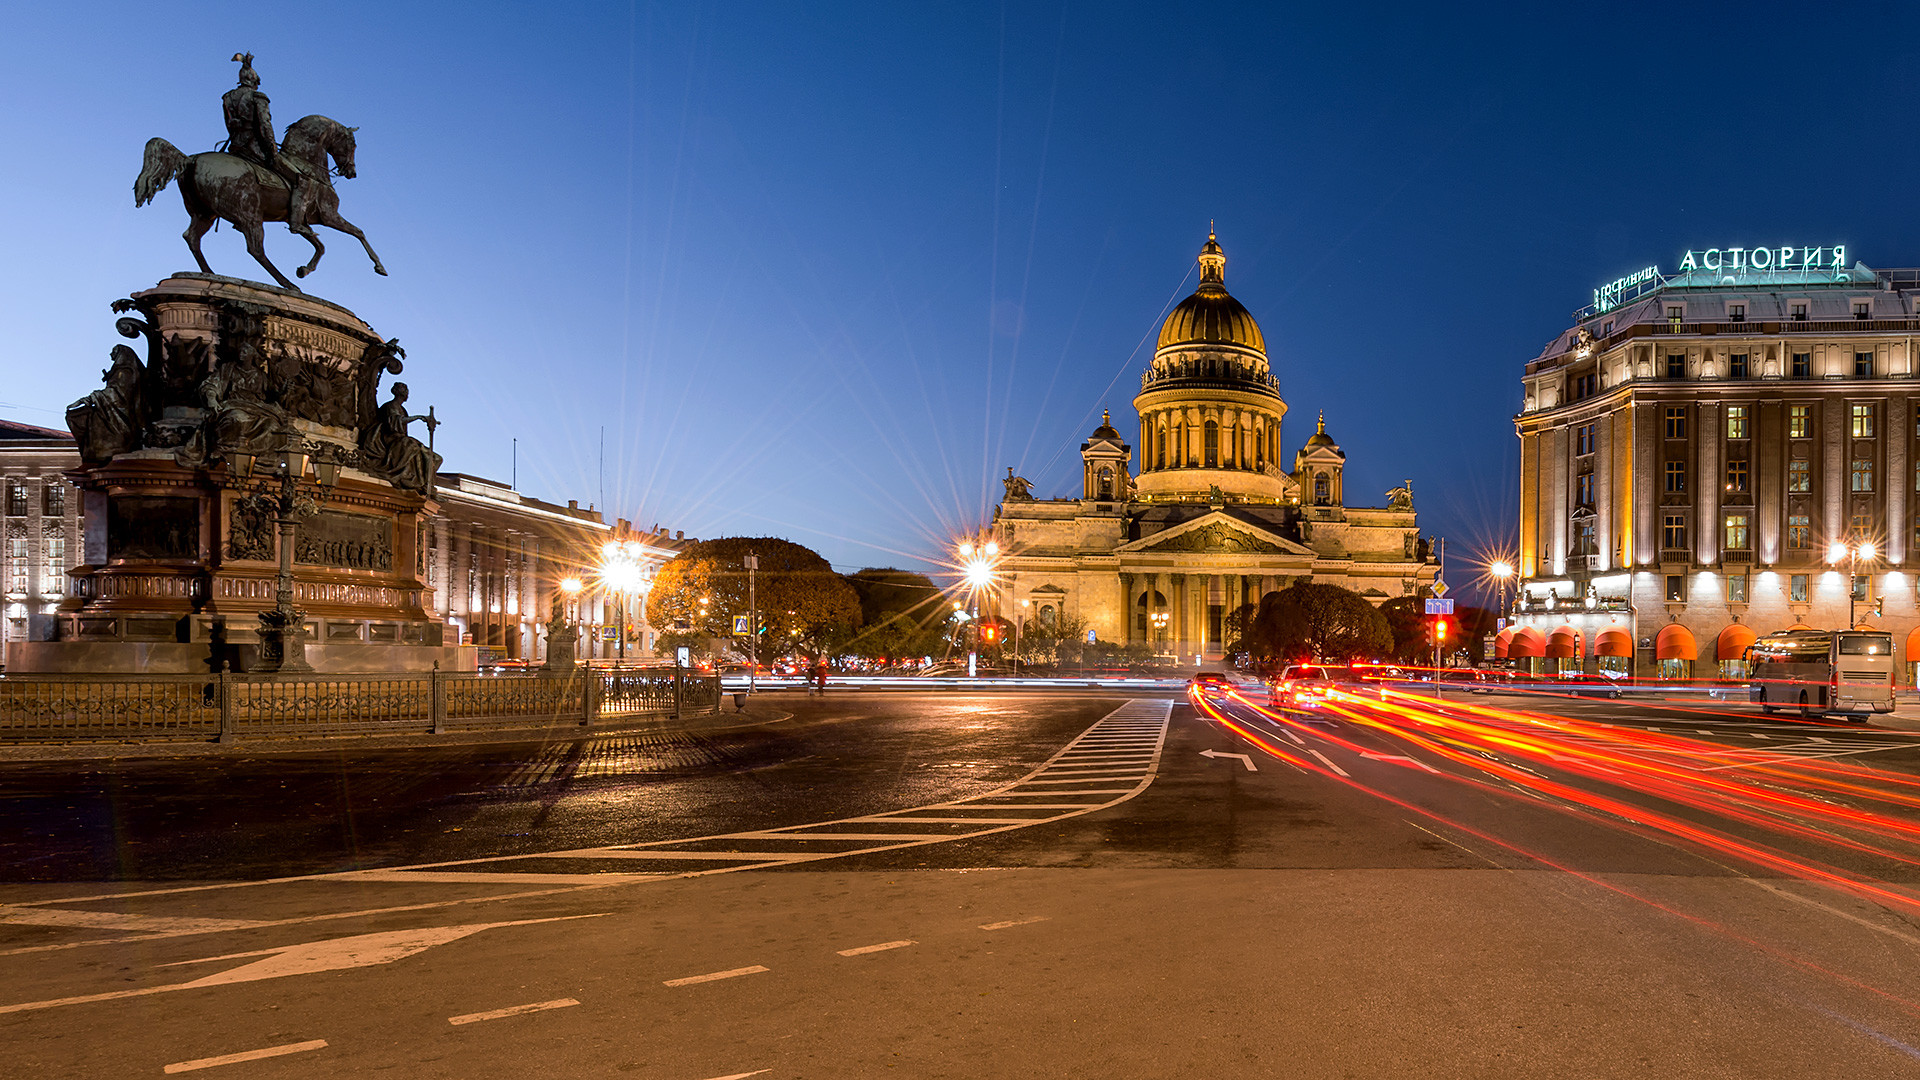
\includegraphics[scale=0.6]{spb}
		\\Saint-Petersburg
	\end{gdblank}
	\begin{gdblank}
		\centering
\includegraphics[scale=0.8]{bigdata} 
	\end{gdblank}
	\begin{gdblank}
		\centering
\includegraphics[scale=0.25]{garchitect} 
		\par\LARGE
		Software Architect
	\end{gdblank}
	\begin{gdblank}
		\frametitle{Data Streaming}
		\centering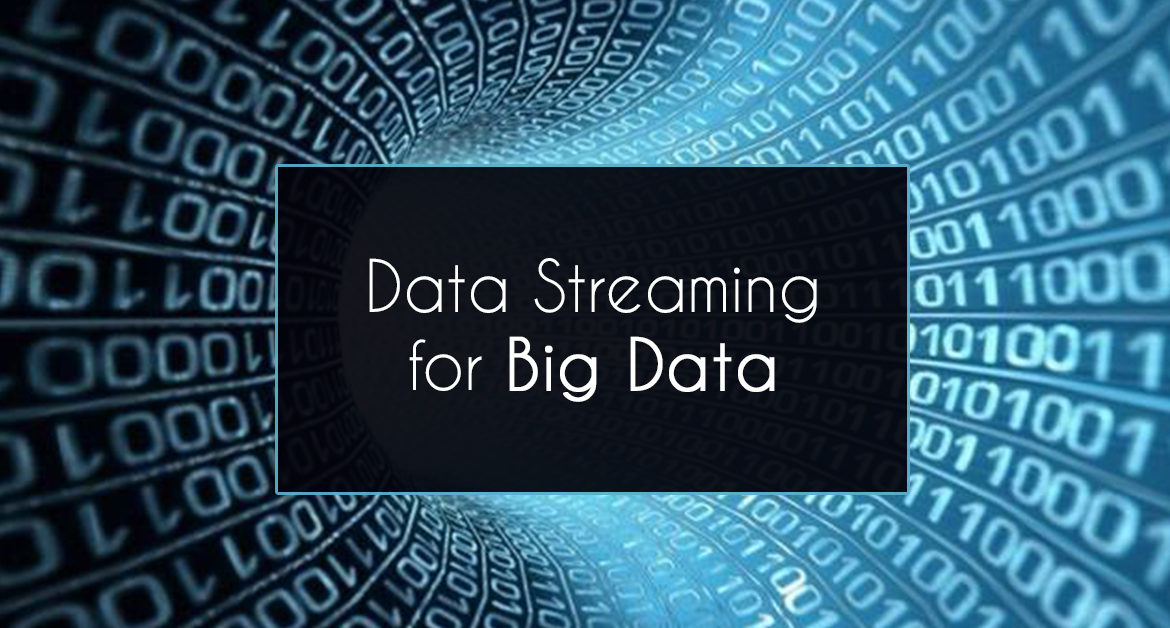
\includegraphics[width=0.8\textwidth]{streaming} 
	\end{gdblank}
	\begin{gdblank}
		\centering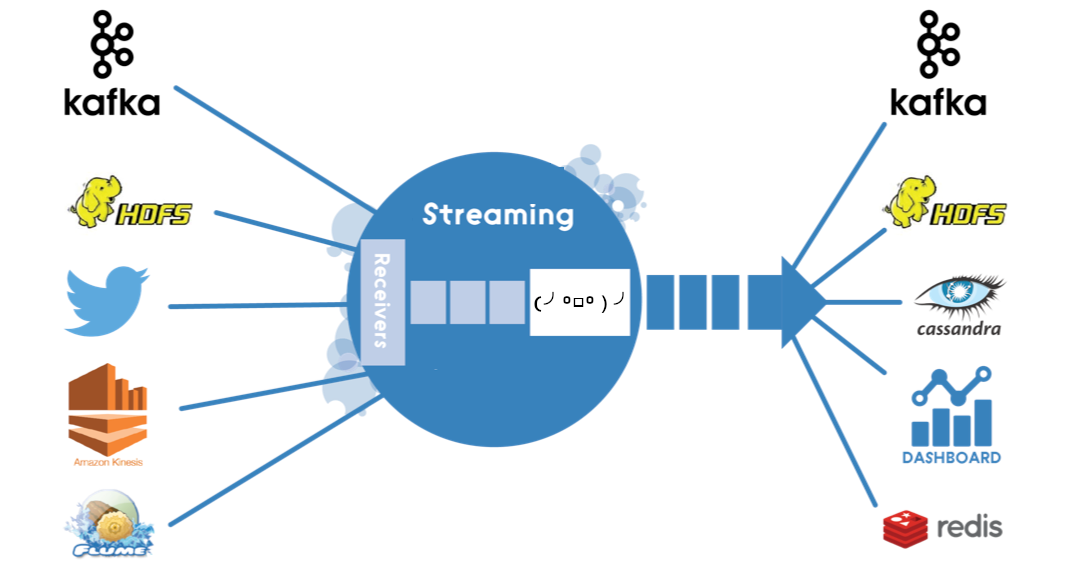
\includegraphics[width=0.9\textwidth]{streaming-details} 
	\end{gdblank}
	\begin{gdblank}
		\centering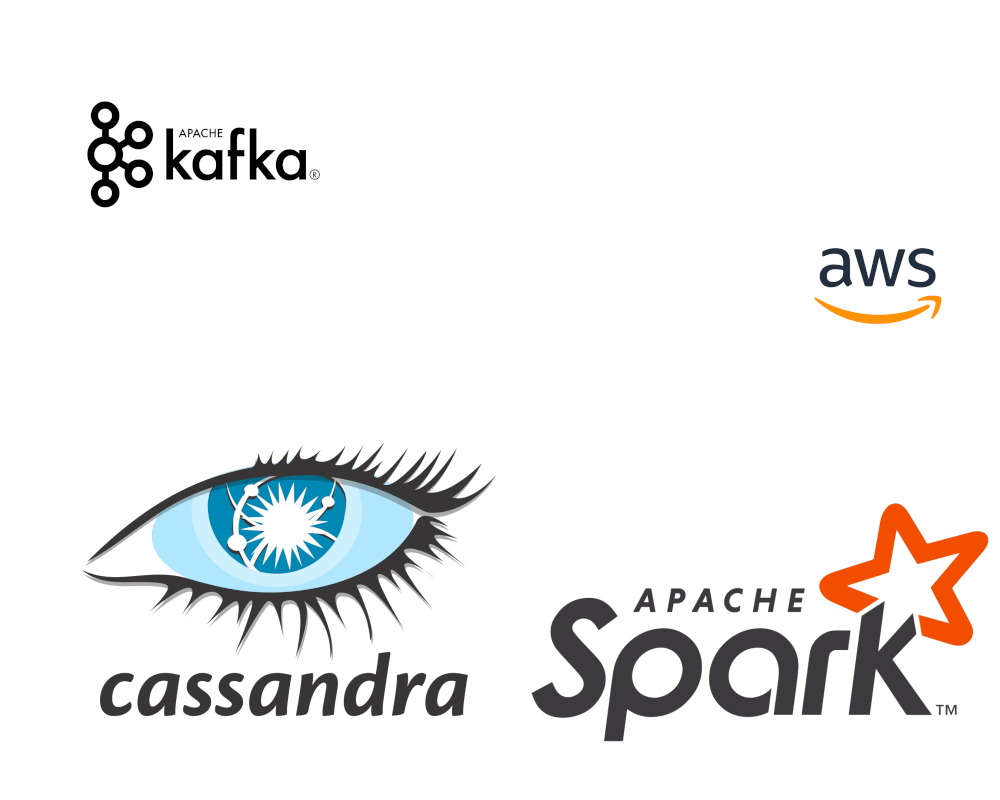
\includegraphics[width=0.7\textwidth]{tech-part} 
	\end{gdblank}
	\begin{gdblank}
		\centering
\includegraphics[width=0.7\textwidth]{tech-all} 
	\end{gdblank}
	\begin{gdblank}
		\frametitle{Big Data School}
		\centering
\includegraphics[scale=0.6]{school}
		\par\LARGE
		\pause
		\textbf{
			Professor
		}		
	\end{gdblank}
	\begin{gdblank}
		\centering{\fontsize{100pt}{120pt}\selectfont\bf Boring}
	\end{gdblank}   
	\begin{gdblank}
		% \frametitle{Hello}
		\begin{columns}
			\begin{column}{0.5\textwidth}
				\centering
\includegraphics[scale=0.6]{bigdata}
			\end{column}
			\pause 
			\begin{column}{0.5\textwidth}
				\centering
\includegraphics[scale=0.23]{gdlogo}
			\end{column}
		\end{columns}        
	\end{gdblank}
	\begin{gdblank}
		\centering
\includegraphics[scale=0.8]{love-job} 
	\end{gdblank}
	\begin{gdblank}
		\frametitle{Time} 
		\begin{columns}
			\begin{column}{0.5\textwidth}
				\centering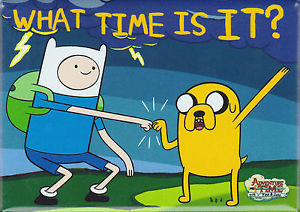
\includegraphics[scale=5]{adventuretime} 
			\end{column}
			\pause 
			\begin{column}{0.5\textwidth}
				\centering
\includegraphics[scale=0.3]{time2} 
			\end{column}
		\end{columns}            
	\end{gdblank}
	\begin{gdblank}
		\frametitle{Time}
		\begin{columns}
			\begin{column}{0.5\textwidth}
				\centering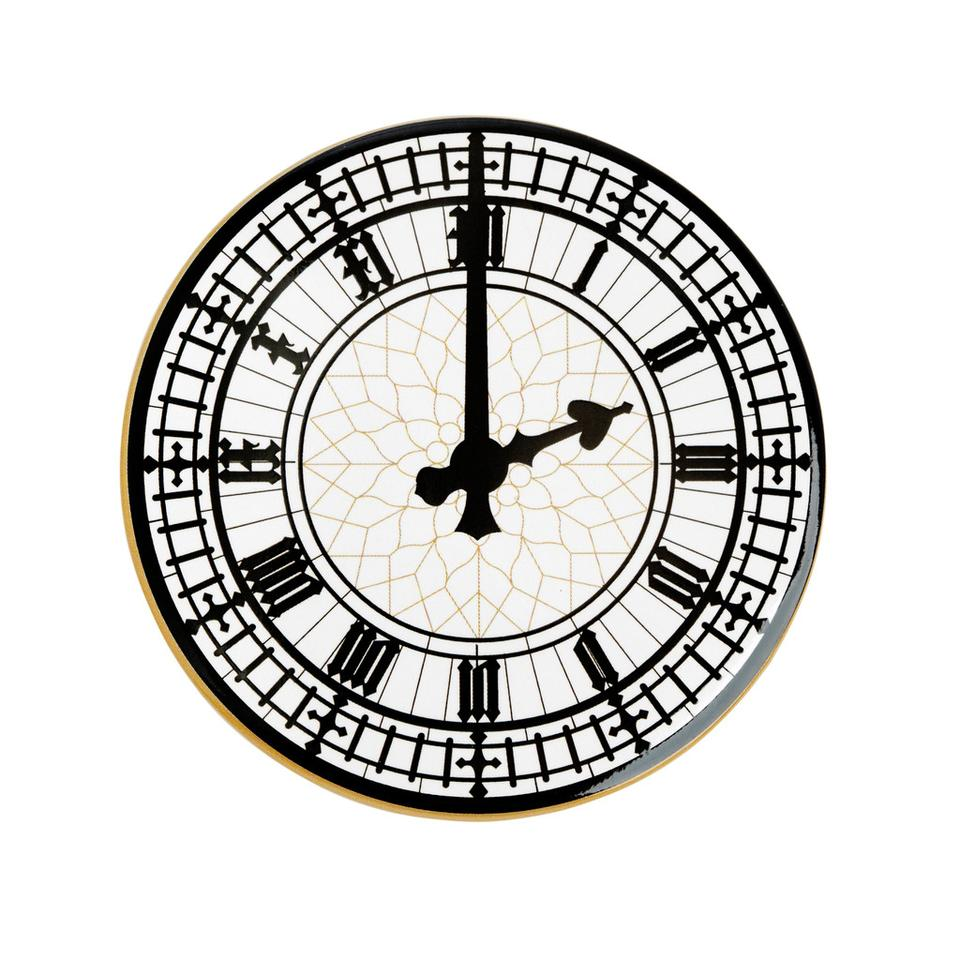
\includegraphics[width=0.9\textwidth]{ordinary-clockface} 
			\end{column}
			\pause 
			\begin{column}{0.5\textwidth}
				\centering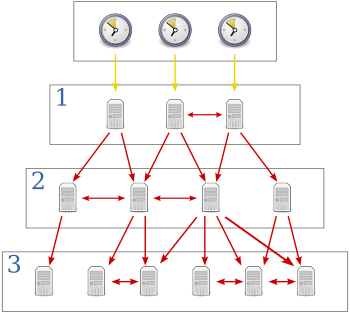
\includegraphics[scale=0.5]{strarum} 
			\end{column}
		\end{columns}            
	\end{gdblank}
	\begin{gdblank}
		\frametitle{Question}
		\centering\Huge What is time?           
	\end{gdblank} 
	\begin{gdblank}
		\frametitle{Time is ...}
		\begin{columns}
			\begin{column}{0.5\textwidth}
				\centering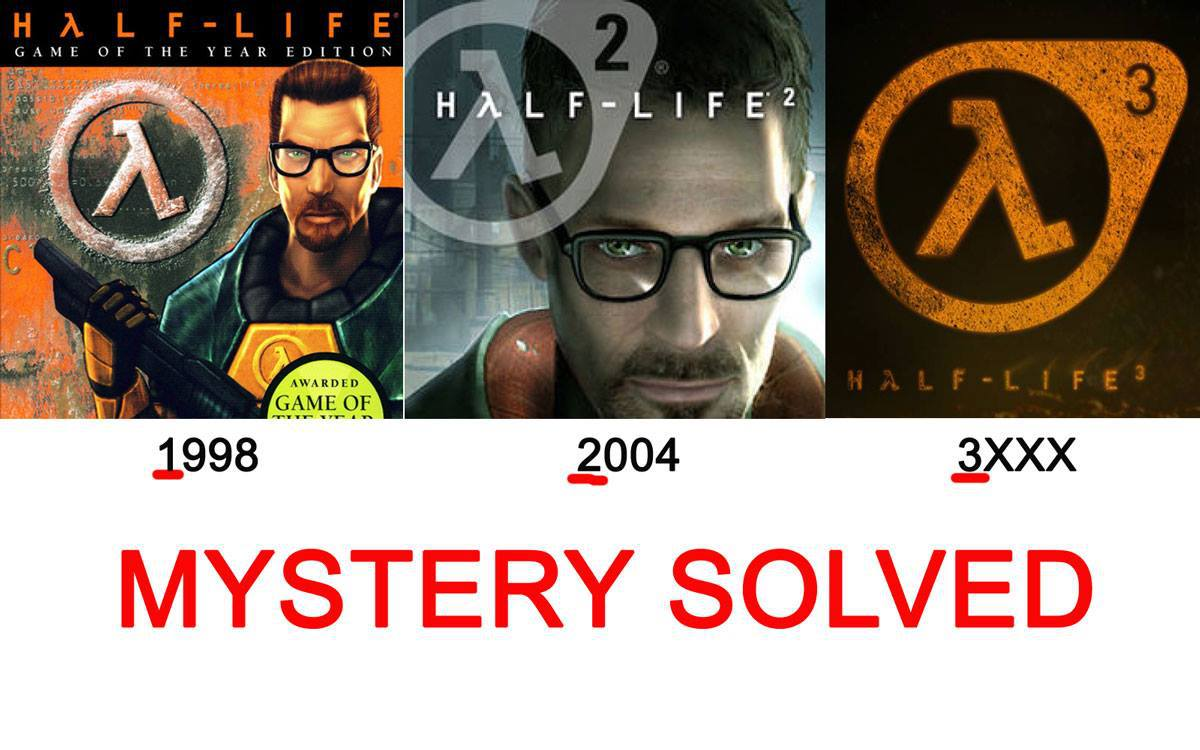
\includegraphics[scale=0.16]{halflife} 
				\\Way of arrange the order of events 
			\end{column}
			\pause 
			\begin{column}{0.5\textwidth}
				\centering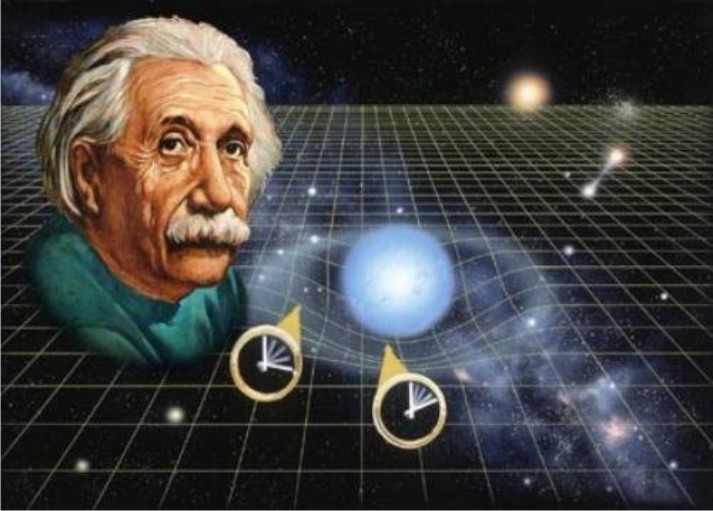
\includegraphics[scale=0.35]{einsteinspacetime} 
				\\Another dimension
			\end{column}
		\end{columns} 
	\end{gdblank} 
	\begin{gdblank}
		\frametitle{Definition of time}
		\LARGE Compact and robust definition of time has proved to be remarkably tricky and elusive.
		\large
		\vskip1cm
		\begin{itemize}
			\item What clocks measure (attr. to physicists Albert Einstein, Donald Ivey, and others)
			\item What prevents everything from happening at once (physicist John Wheeler and others)
			\item A linear continuum of instants (philosopher Adolf Grünbaum)
		\end{itemize}
	\end{gdblank}
	% \begin{gdblank}
	% 	\frametitle{Religion}
	% 	\begin{columns}
	% 		\begin{column}{0.5\textwidth}
	% 			\centering
\includegraphics[width=0.9\textwidth]{pray} 
	% 		\end{column}
	% 		\begin{column}{0.5\textwidth}
	% 			\begin{block}{Wikipedia}
	% 				In Zurvanism, Zurvan was perceived as the god of infinite time and space and was aka ("one", "alone").
	% 			\end{block} 
	% 		\end{column}
	% 	\end{columns}     
	% \end{gdblank}
	\begin{gdblank}
		\frametitle{Time is ...}
		\LARGE\centering Time is something we deal with every day, and something that everyone thinks they 
		\bf understand
	\end{gdblank} 
	\begin{gdblank}
		\begin{columns}
			\begin{column}{0.5\textwidth}
				\centering
\includegraphics[width=\textwidth]{adventure} 
			\end{column}
			\begin{column}{0.5\textwidth}
				\Huge\centering Game time! 
			\end{column}
		\end{columns}     		
	\end{gdblank} 
	\begin{gdblank}
		\frametitle{Round 1}    
		\begin{columns}
			\begin{column}{0.70\textwidth}
				\centering
				\LARGE There are always 24 hours in a day 
				\pause     
			\end{column}
			\begin{column}{0.3\textwidth}
				\large\centering Daylight saving time 
				\vskip0.5cm
				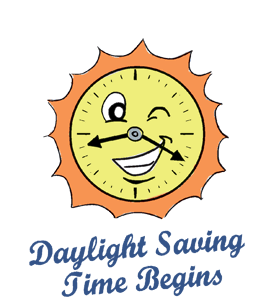
\includegraphics[scale=0.5]{daylightsaving}
			\end{column}
		\end{columns}
	\end{gdblank} 
	
	\begin{gdblank}
		\begin{columns}
			\frametitle{Round 2}    
			\begin{column}{0.70\textwidth}
				\centering
				\LARGE There are 60 seconds in a minute 
				\pause     
			\end{column}
			\begin{column}{0.3\textwidth}
				\large\centering Leap Second
				\vskip0.5cm
				
\includegraphics[width=0.9\textwidth]{leapsecond}
			\end{column}
		\end{columns}
	\end{gdblank}
	\begin{gdblank}
		\frametitle{Round 3}    
		\begin{columns}
			\begin{column}{0.70\textwidth}
				\centering
				\LARGE A month always ends in the same year it started
				\pause     
			\end{column}
			\begin{column}{0.3\textwidth}
				\large\centering 
				\begin{itemize}
					\item Fiscal year/calendar
					\item Chinese Year
				\end{itemize}
				\vskip0.5cm
				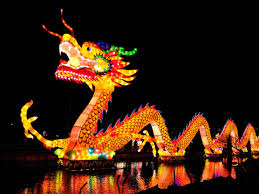
\includegraphics[scale=0.5]{china}
			\end{column}
		\end{columns}
	\end{gdblank} 
	\begin{gdblank}
		\frametitle{Round 4}    
		\begin{columns}
			\begin{column}{0.70\textwidth}
				\centering
				\LARGE Month could have less than 20 days
				\pause     
			\end{column}
			\begin{column}{0.3\textwidth}
				\large\centering  September 1752 had 19 days in British Empire
				\vskip0.5cm
				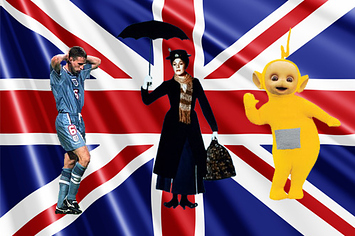
\includegraphics[scale=0.35]{british}
			\end{column}
		\end{columns}
	\end{gdblank} 
	\begin{gdblank}
		\frametitle{Everyone's do it wrong!}
		\centering{\fontsize{140pt}{150pt}\selectfont\bf ?}
	\end{gdblank}   
	\begin{gdblank}
		\begin{columns}
			\begin{column}{0.5\textwidth}
				
\includegraphics[width=\textwidth]{aliens}				

			\end{column}
			\pause
			\begin{column}{0.5\textwidth}
				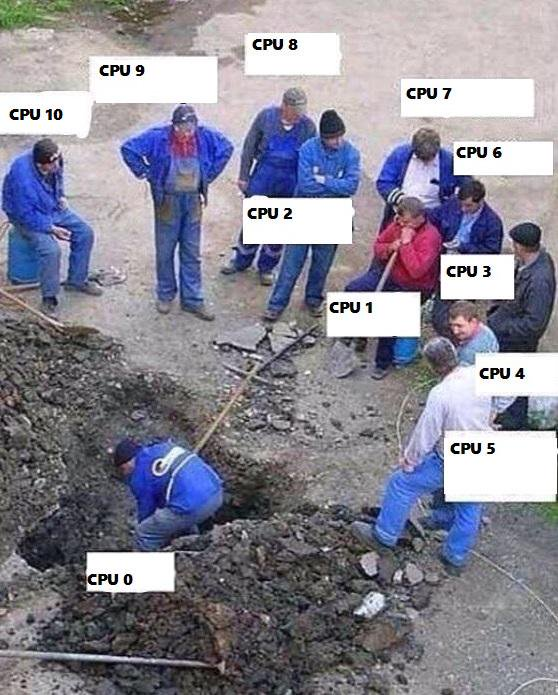
\includegraphics[width=\textwidth]{cpu}
			\end{column}
		\end{columns}				
	\end{gdblank}  
	\begin{gdblank}		
		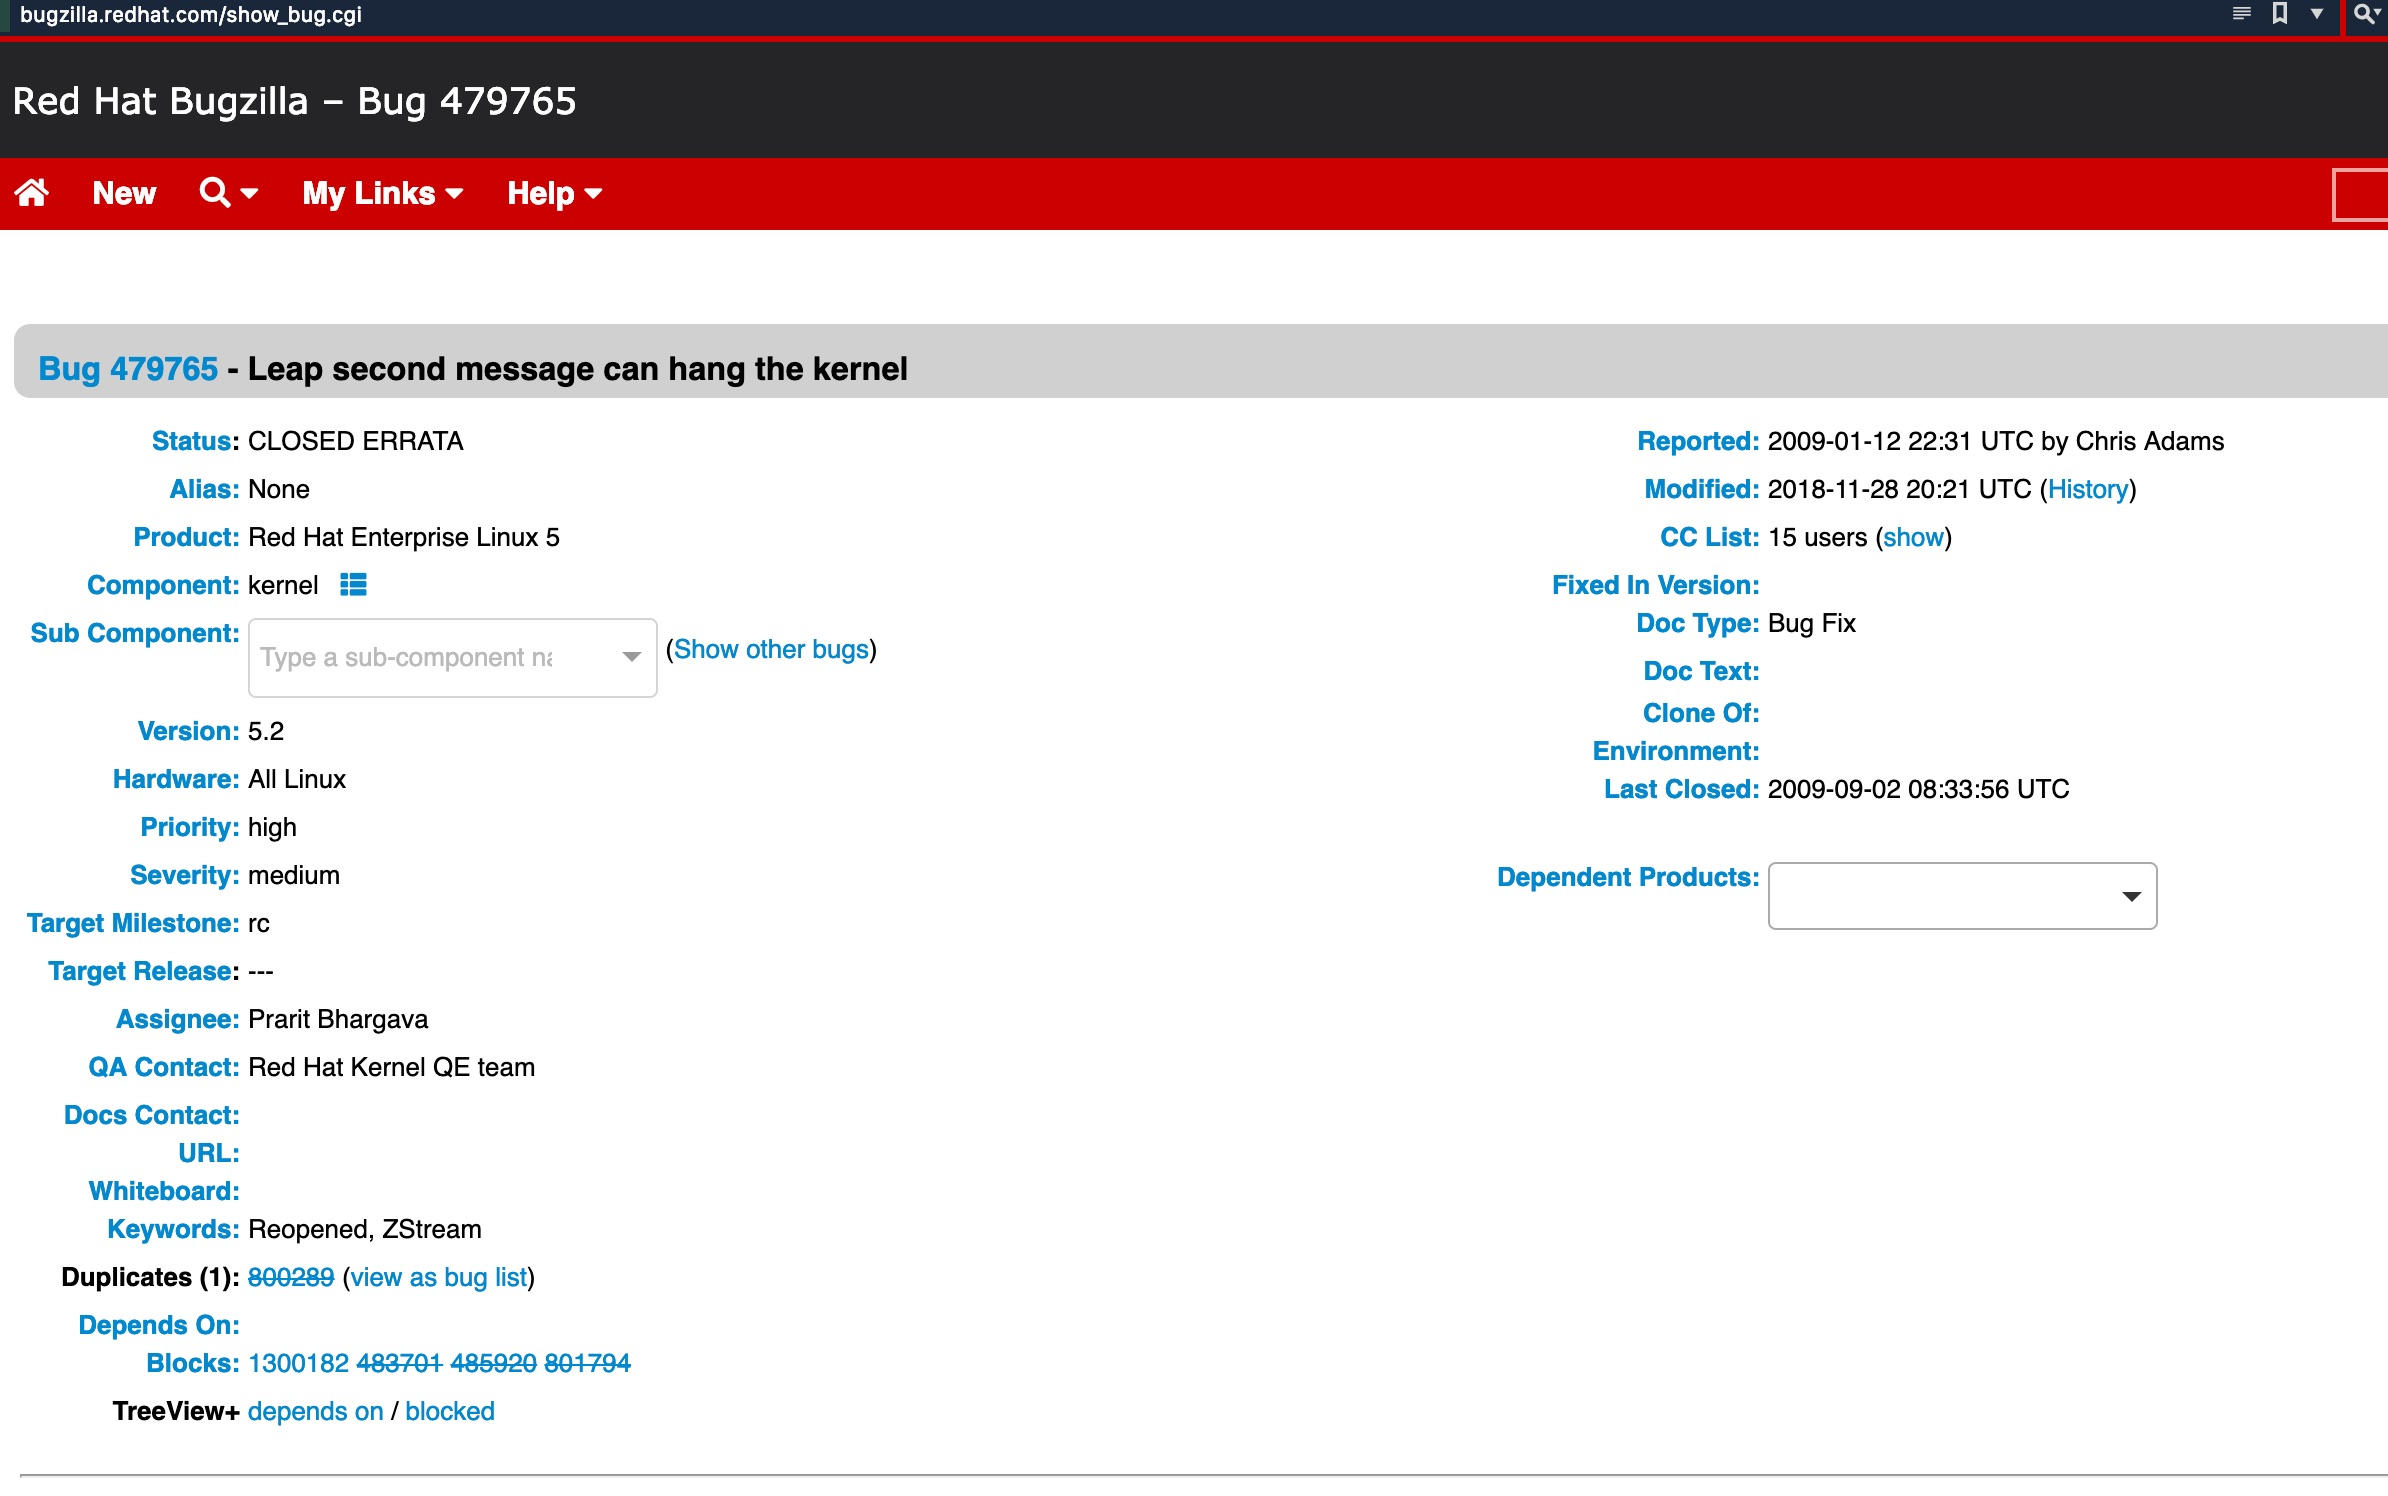
\includegraphics[width=\textwidth]{kernel-time-bug}
	\end{gdblank}  
	\begin{gdblank}		
		\frametitle{Java Code}
		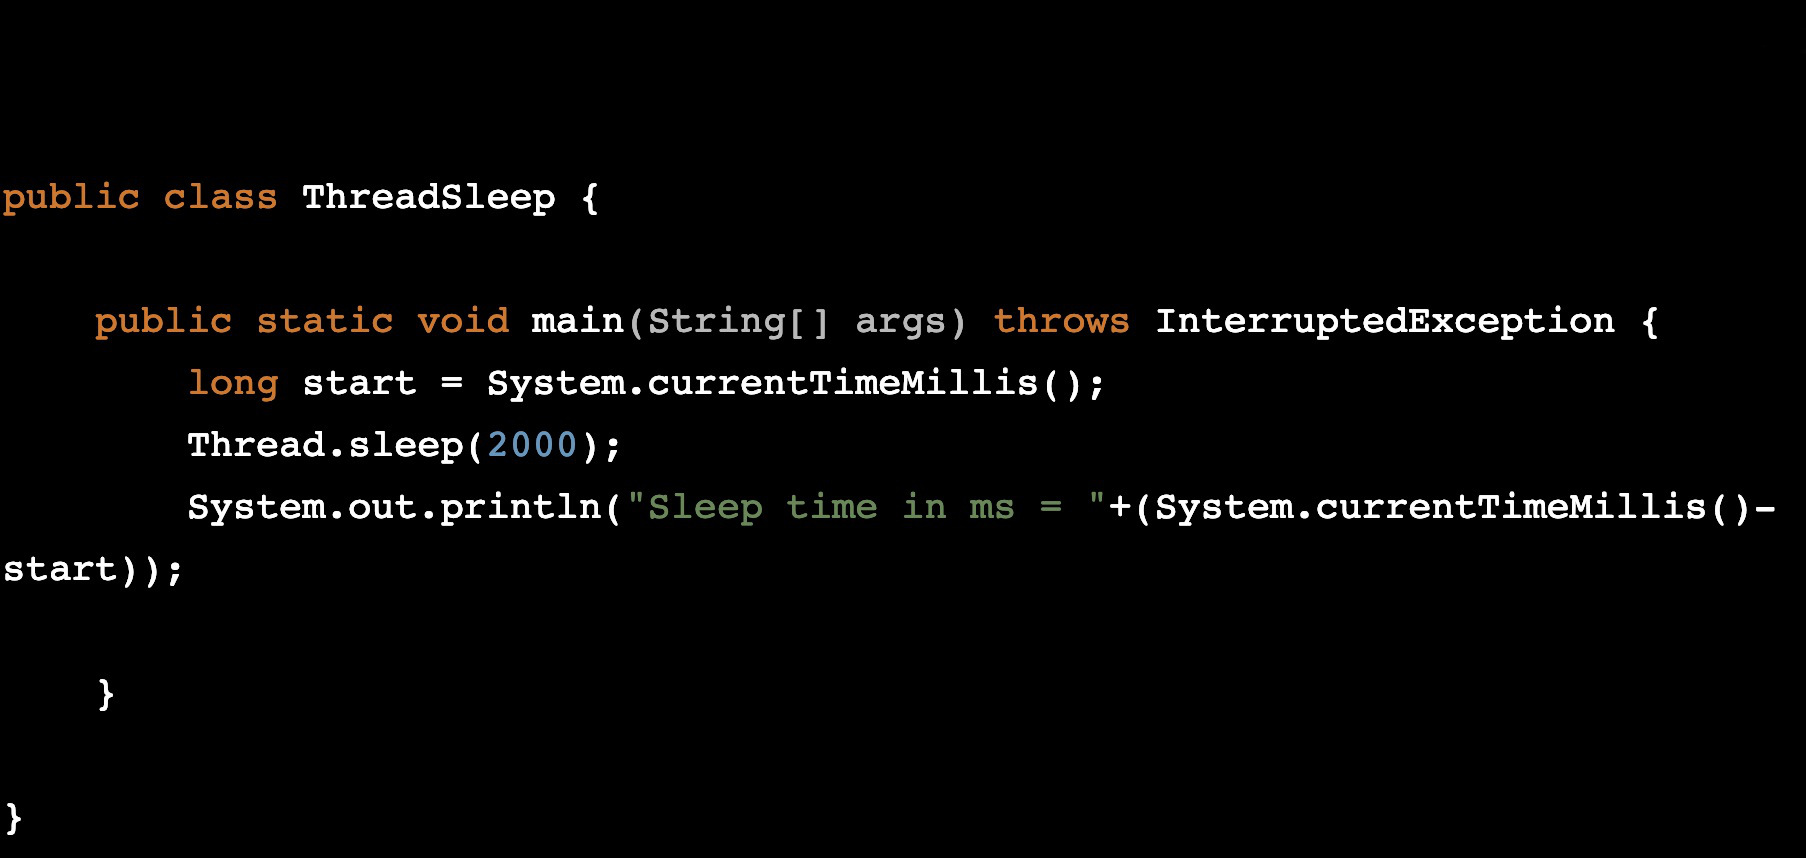
\includegraphics[width=\textwidth]{sleep}
	\end{gdblank}   
	\begin{gdblank}
		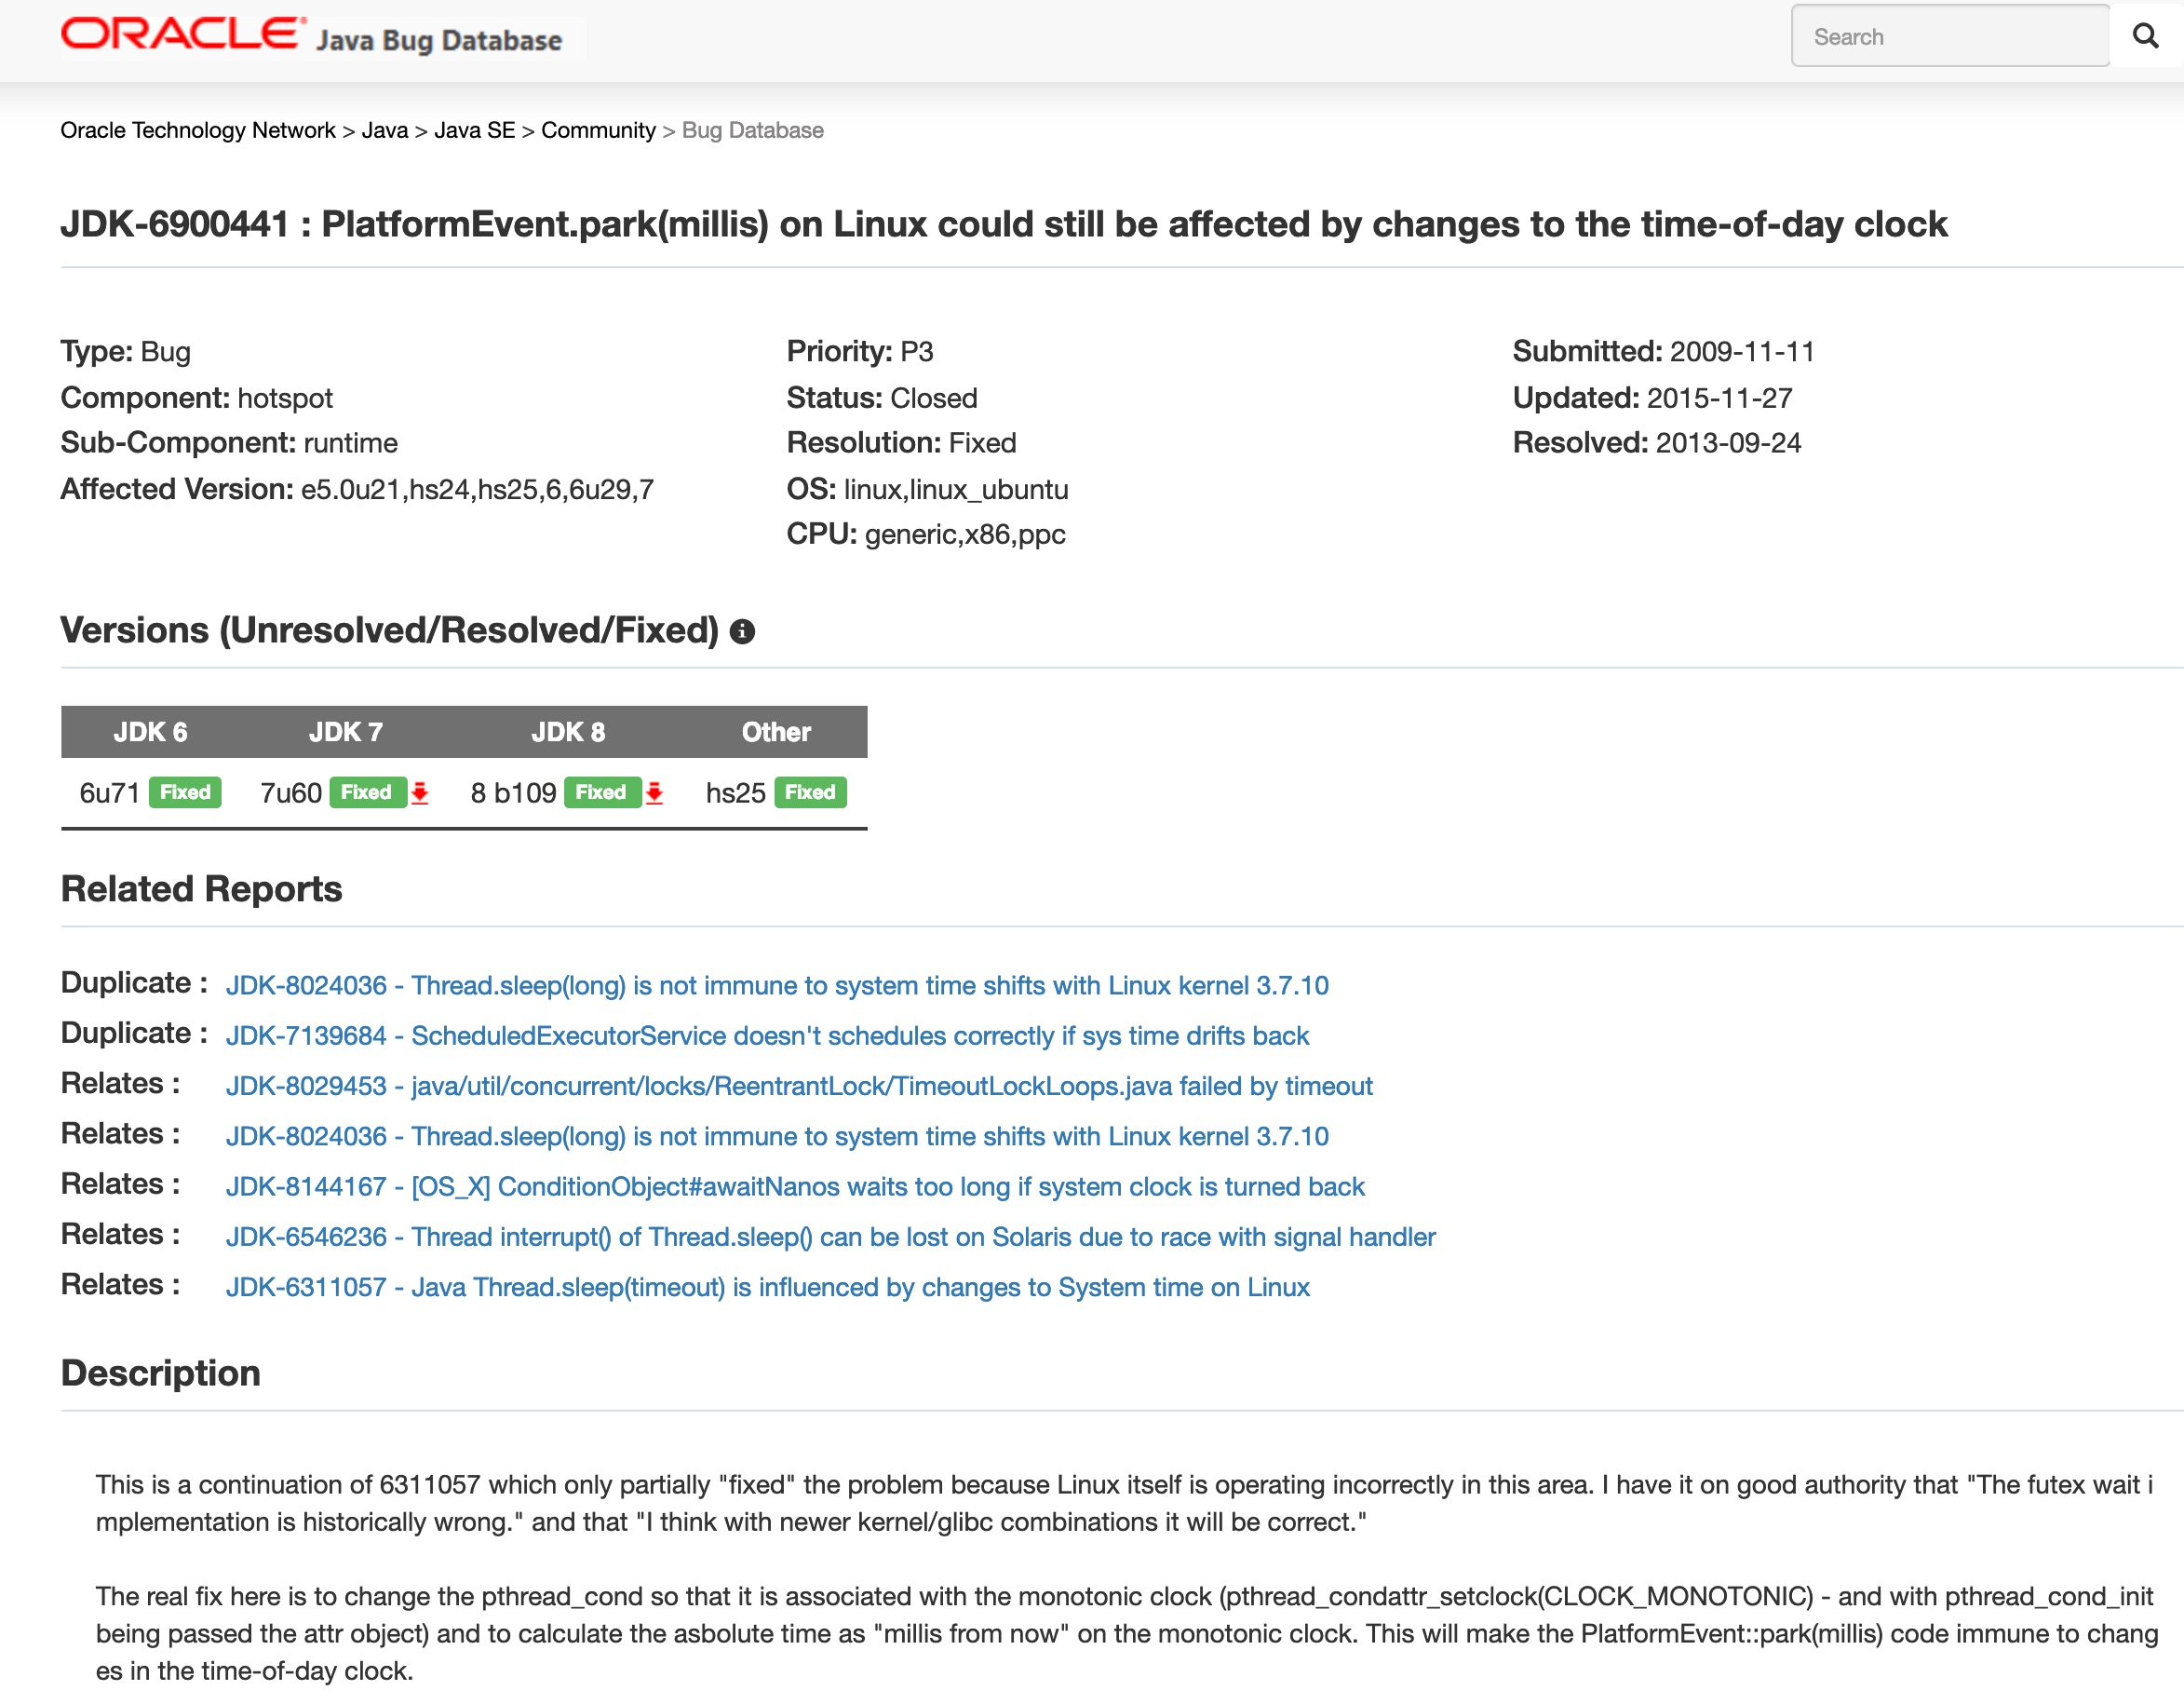
\includegraphics[width=\textwidth]{jvm-time-bug}
	\end{gdblank}
	\begin{gdblank}
		\frametitle{Distributed environment}
		\centering
		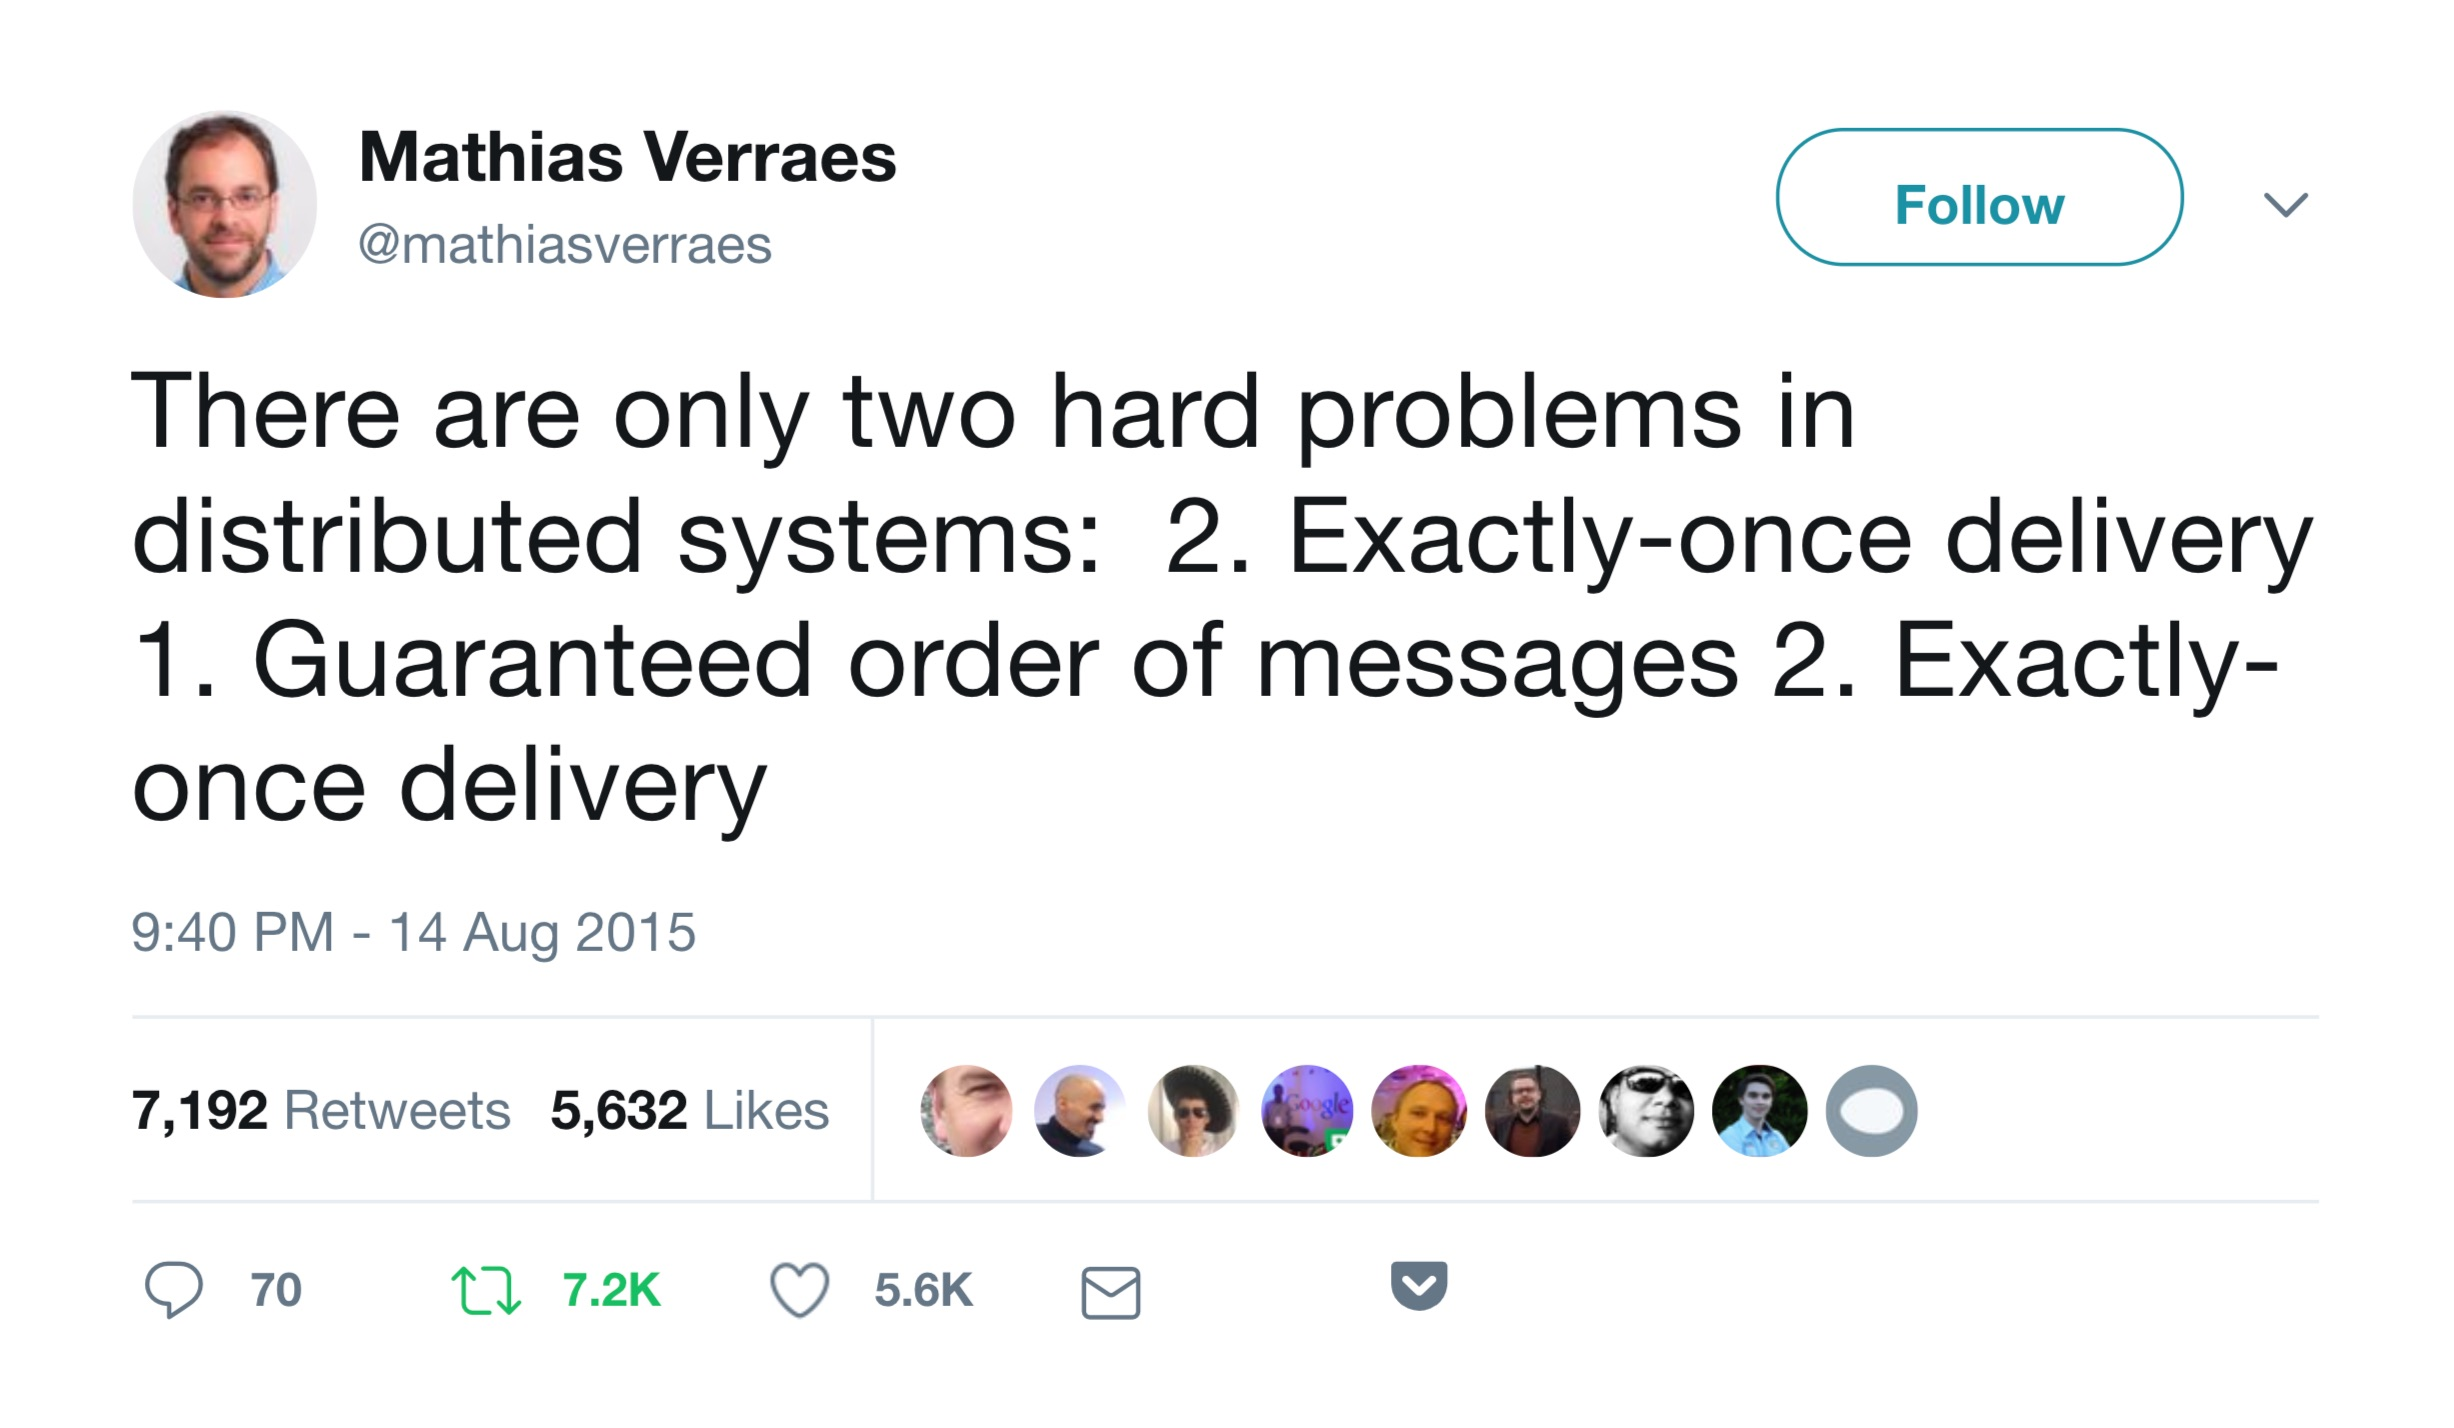
\includegraphics[width=0.9\textwidth]{2-problems}
	\end{gdblank}
	\begin{gdblank}
		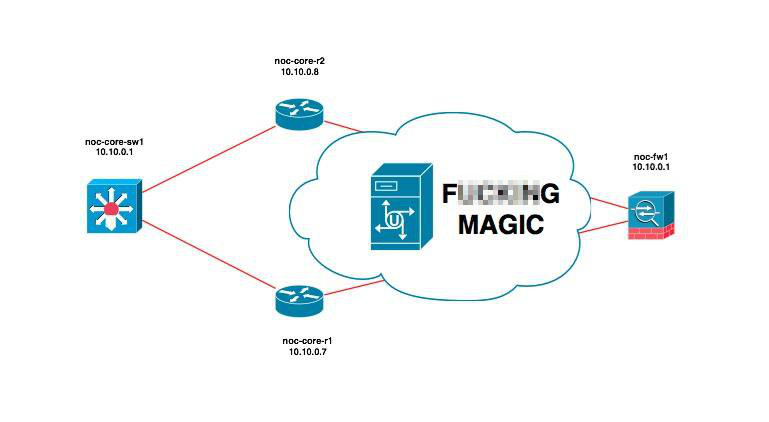
\includegraphics[width=\textwidth]{networkb}
	\end{gdblank}   
	\begin{gdblank}
		\begin{columns}
			\begin{column}{0.6\textwidth}
				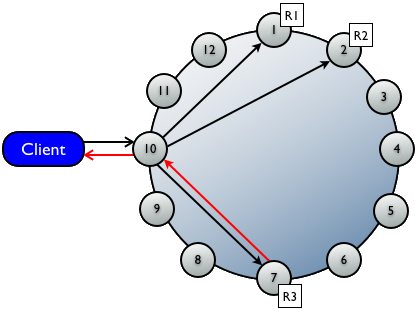
\includegraphics[width=\textwidth]{cassandrawrite}
			\end{column}
			\begin{column}{0.4\textwidth}
				
\includegraphics[width=\textwidth]{cassandra}
				\centering
				\begin{itemize}
					\item Peer to Peer Database
					\item Masterless Architecture
				\end{itemize}
				\tiny its difficult to reason about events in this system
			\end{column}
		\end{columns}
	\end{gdblank}   
	\begin{gdblank}
		\frametitle{I am the Law and Order}
		\centering
		
\includegraphics[scale=0.22]{order}
		\\Needed to establish the order of events that have occurred in the system or when they will occur in the future
	\end{gdblank}
	\begin{gdblank}
		\frametitle{Order in Chaos}
		\LARGE
		\begin{itemize}
			\item Maintain consistency
			\item Build reliable systems
			\item Mutual exclusions
			\item Debug [Resumption of execution]
		\end{itemize}
	\end{gdblank}
	\begin{gdblank}
		\frametitle{Common Clock}
		\LARGE
		We can reliably define
		\begin{itemize}
			\item simultaneous: all events that happen between clock ticks
			\pause
			\item before: an event that happens in a previous clock tick
			\item after: an event that happens in a subsequent clock tick
		\end{itemize}
	\end{gdblank}
	\begin{gdblank}
		\frametitle{Distributed Systems}
		\LARGE
		Synchronization in distributed systems is \bf hard
		\begin{itemize}
			\item No shared memory
			\item No common clock
		\end{itemize}
	\end{gdblank}
	\begin{gdblank}
		\frametitle{Wall Clock}		
		\centering
		\LARGE	
		Let's use 'Wall Clocks' and NTP!?
		\par
		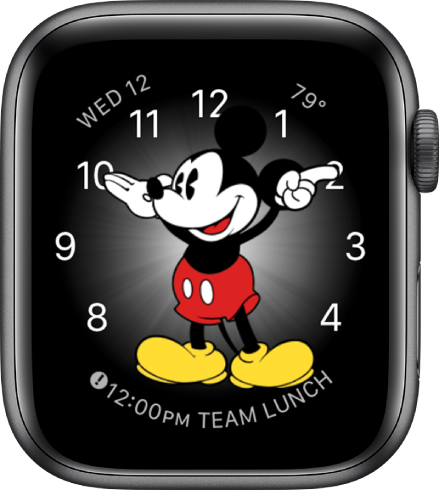
\includegraphics[scale=0.20]{clock}
		\small
		\\When kept under tension the quartz crystal oscillates at a well-defined frequency
	\end{gdblank}
	\begin{gdblank}
		\frametitle{Clock Drift}
		\begin{columns}
			\begin{column}{0.6\textwidth}
				We can't have perfect clocks
				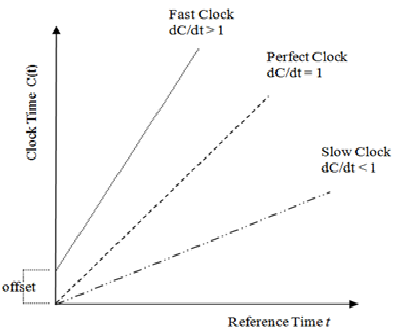
\includegraphics[scale=0.5]{clockdrift}
			\end{column}
			\begin{column}{0.4\textwidth}
				Ordinary clocks drift by about 1 sec in 10 days
			\end{column}
		\end{columns}
	\end{gdblank}
	\begin{gdblank}
		\frametitle{Clock Skew}
		\centering
		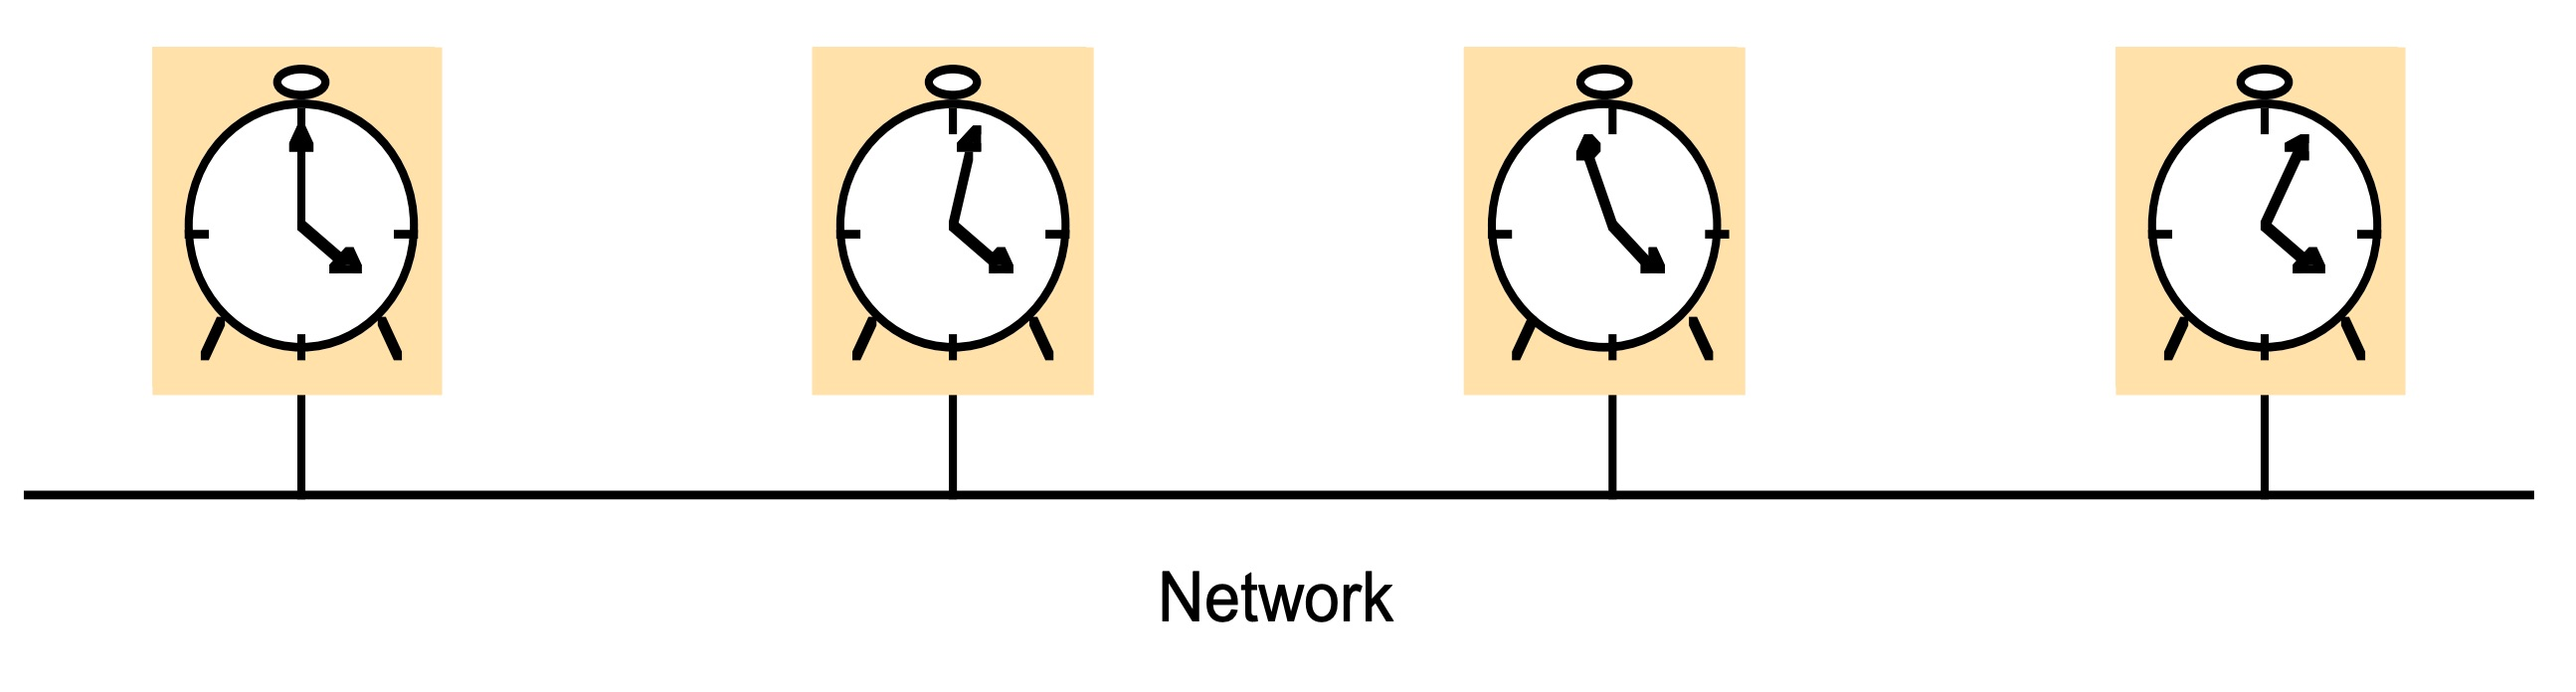
\includegraphics[scale=0.15]{skew}
		\\Skew: the difference between the times on two clocks (at any instant)
	\end{gdblank}
	\begin{gdblank}
		\frametitle{I'm running NTP. I'm good}
		\centering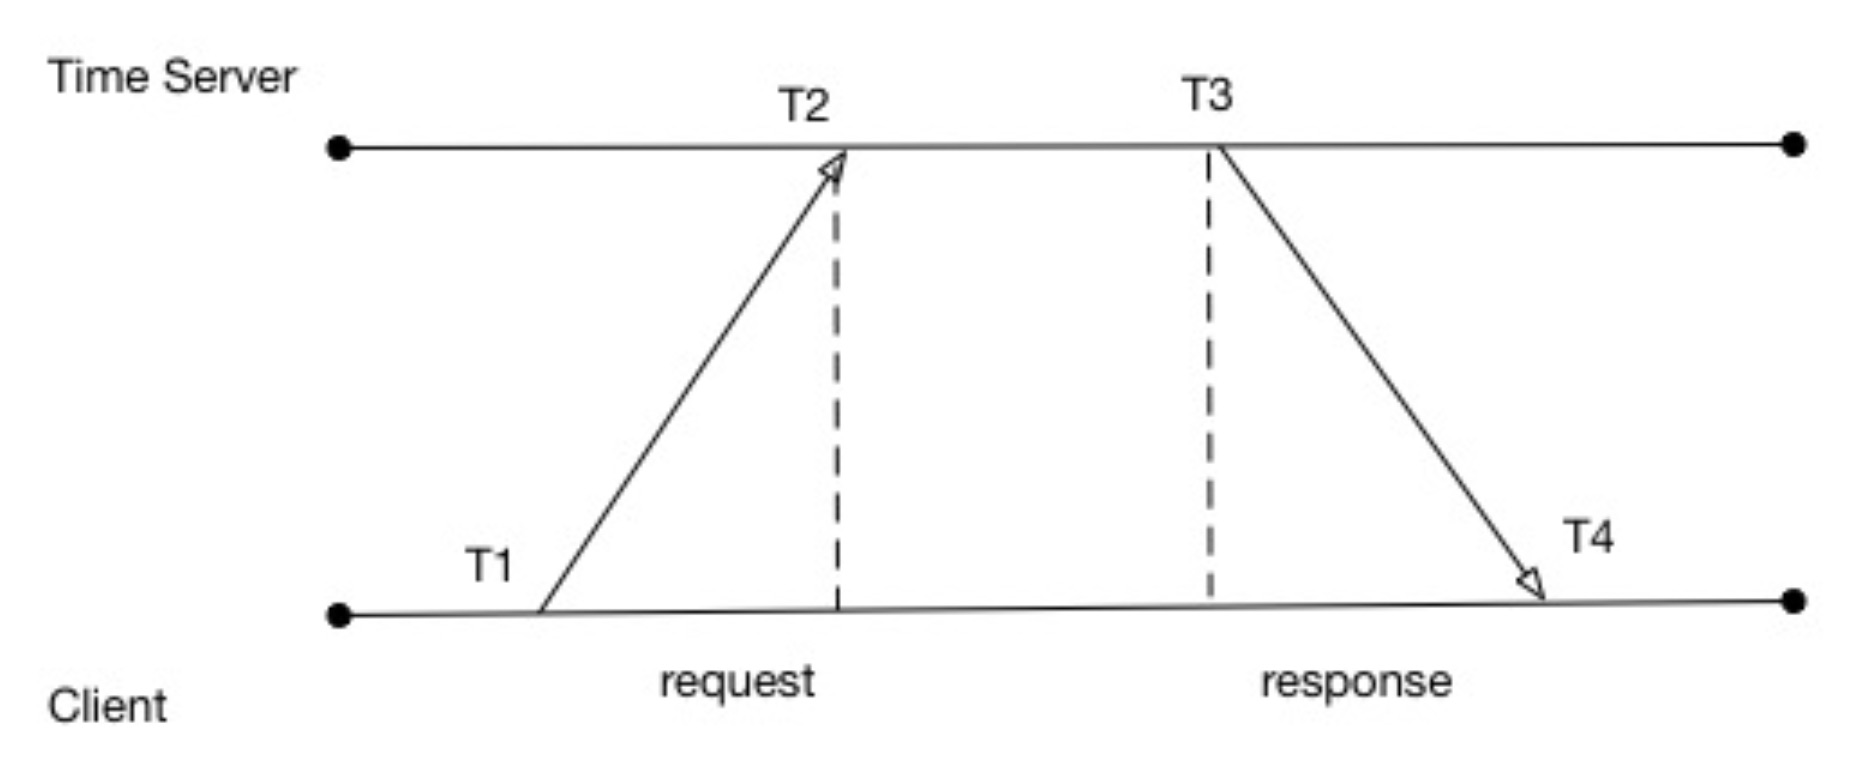
\includegraphics[scale=0.15]{ntp}
		\par
		The challenge with this approach is that there is a delay in the transmission from the time server to the client receiving the time update
		\\This \textbf{delay is not constant for all requests}. Some request may be faster and others slower
	\end{gdblank}
	\begin{gdblank}
		\frametitle{I'm running NTP. I'm good}
		\centering													   
		\LARGE
		\alt<2>{1 / 600000 = 0.0000016 ... microsecond?}{600000 events per second} 
	\end{gdblank}
	\begin{gdblank}
		\frametitle{I'm running NTP. I'm good}
		\centering
		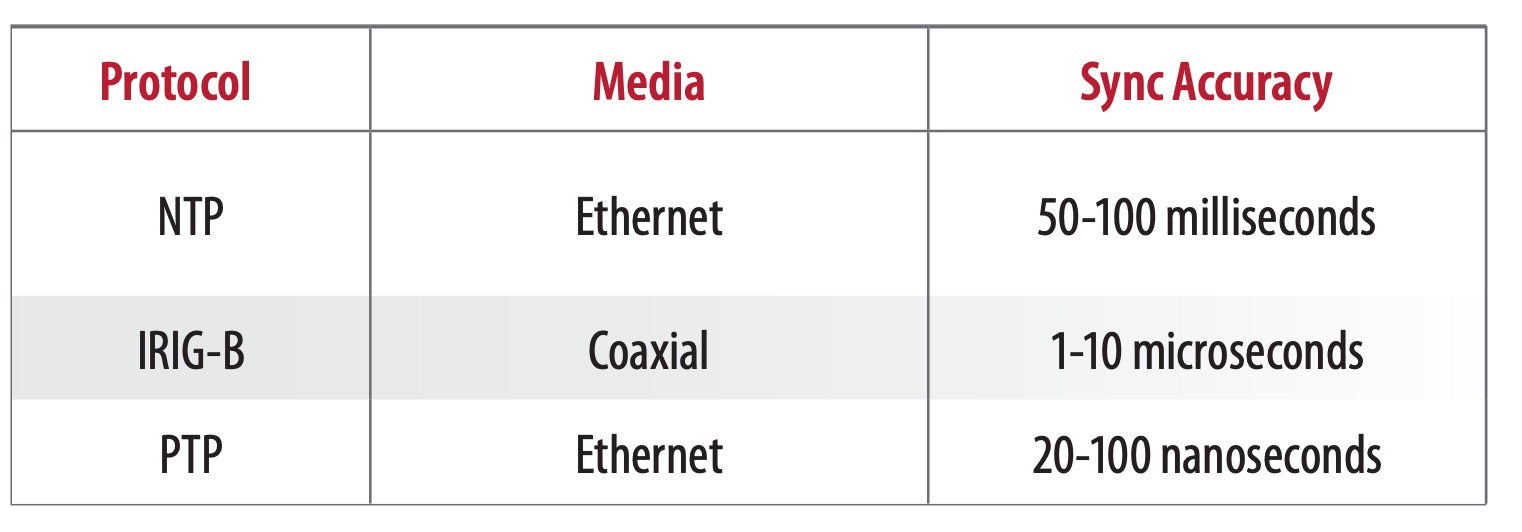
\includegraphics[scale=0.20]{accuracy}
		\\\tiny
		* Choosing the correct Time Synchronization Protocol and incorporating the 1756-TIME module into your Application \\ By: Josh Matson
	\end{gdblank}
	\begin{gdblank}
		\frametitle{Boom!}
		\centering
		% \LARGE It's difficult! \par
		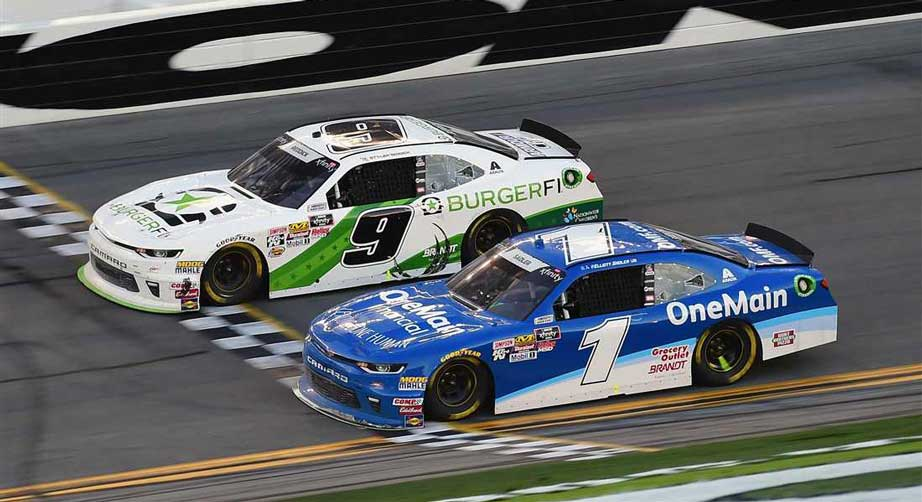
\includegraphics[height=0.6\textheight]{photofinish}
		\large \\
		Correction of time does not mean that all machines agree on time, it just means they are much \textbf{closer to each other on average}
	\end{gdblank}
	\begin{gdblank}
		\frametitle{Leslie Lamport}
		\centering
		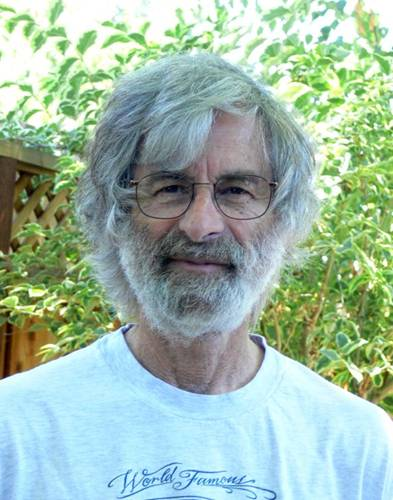
\includegraphics[height=0.6\textheight]{lamport} \\
		\large
		Lamport, L. (1978). "Time, clocks, and the ordering of events in a distributed system"
	\end{gdblank}
	\begin{gdblank}
		\centering
		\begin{itemize}
			\item The important contribution of Lamport is that in a distributed system, \textbf{clocks need not be synchronized absolutely}
			\item It is \textbf{not important} that all \textbf{processes agree on what the actual time is, but that they agree on the order in which events occur}
			\item Happens Before
		\end{itemize}		
	\end{gdblank}
	\begin{gdblank}
		\frametitle{Happens Before}
		The relation '\rightarrow' on the set of events of a system is a smallest relation satisfying three conditions
		\begin{itemize}
			\item If $a$ and $b$ are events \textbf{in the same process}, and $a$ comes before $b$, then $a$ \rightarrow $b$ 
			\item If $a$ is the sending of a message by one process and $b$ is the receipt of the same message by another process, then $a\rightarrow b$
			\item Transitive. If $a\rightarrow b$ and $b\rightarrow c$ then $a\rightarrow c$. Two distinct events $a$ and $b$ are said to be concurrent if $a\cancel{\rightarrow} b$ and $b\cancel{\rightarrow} a$
		\end{itemize}				
		\par
		If $a\rightarrow b$ happens between \textbf{two process}, and events $x$ and $y$ occur on another set of processes and these two sets of processes don’t exchange messages then:\\
		we cannot say whether $x\rightarrow y$ or $y\rightarrow x$ from the perspective of the first set of processes
		\tiny outcome
	\end{gdblank}
	\begin{gdblank}
		\frametitle{Example}
		\begin{columns}
			\begin{column}{0.5\textwidth}
				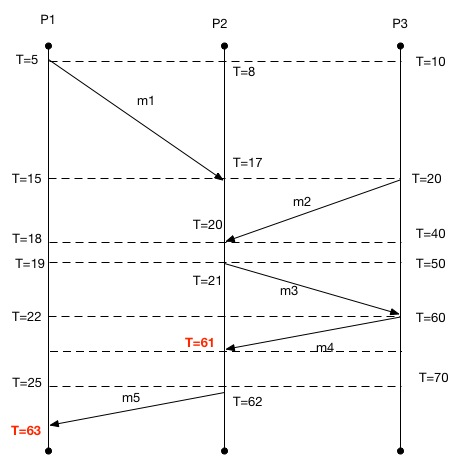
\includegraphics[height=0.85\textheight]{lamport_clocks_dia}			
			\end{column}
			\begin{column}{0.5\textwidth}
				\begin{itemize}
					\item When a message is transmitted from $P1 \rightarrow P2$, $P1$ will encode the send time into the message
					      \pause
					\item When $P2$ receives the message, it will record the time of receipt
					      \pause
					\item If the time at $P2$ is already greater than the send time, then no action is required for $P2$
					      \pause
					\item If $P2$ discovers that the time of receipt is before the send time, $P2$ will update its software clock to be one greater than the send time
					      \pause
					\item “happens-before” relationship is preserved with this actions
				\end{itemize}
			\end{column}	
		\end{columns}
	\end{gdblank}
	\begin{gdblank}
		\frametitle{Lamport Clocks Limitations}
		\centering
		\large		
		With Lamport’s clocks nothing can be said about \textbf{the actual time} of a and b.
	\end{gdblank}
	\begin{gdblank}
		\frametitle{Causality} 
		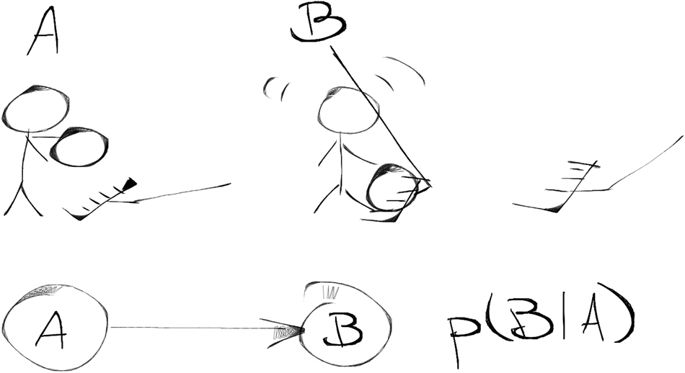
\includegraphics[scale=0.4]{causality}
		\centering\\Causal relations\\An example of a causal relation and its representation in a graph. 
		\tiny \\Credits: C. Giarmatzi
	\end{gdblank}   
	\begin{gdblank}
		\frametitle{Who did when?}
		\begin{columns}
			\begin{column}{0.5\textwidth}
				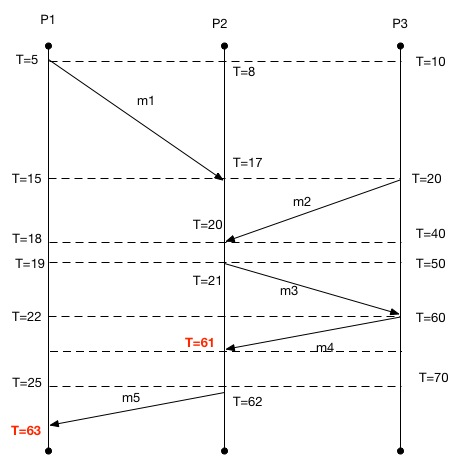
\includegraphics[height=0.8\textheight]{lamport_clocks_dia}			
			\end{column}
			\begin{column}{0.5\textwidth}
				\begin{itemize}
					\item $m1 \rightarrow m3$?
					\item $m2 \rightarrow m3$? 
				\end{itemize}
			\end{column}	
		\end{columns}
	\end{gdblank}
	\begin{gdblank}
		\frametitle{Vector Clocks}
		\centering
		\LARGE
		Vector Clocks
		\par\large
		by Colin Fidge and Friedemann Mattern in 1988
	\end{gdblank}
	\begin{gdblank}
		\frametitle{Vector Clocks}
		\centering
		\large
		\begin{itemize}
			\item A vector clock of a system of N processes is \textbf{an array/vector} of N logical clocks, \textbf{one clock per process}
			\item A vector clock $VC(a)$ is assigned to an event $a$
			\item If $VC(a)<VC(b)$ for events $a$ and $b$, then event $a$ is known to causally precede $b$
		\end{itemize}
	\end{gdblank}
	\begin{gdblank}
		\frametitle{Robbery}
		\begin{columns}
			\begin{column}{0.5\textwidth}
				
\includegraphics[width=0.9\textwidth]{robbery}			
			\end{column}
			\begin{column}{0.5\textwidth}
				Alice, Ben, Cathy, and Dave want to rob a bank
				\begin{itemize}
					\item They could send P2P messages
					\item No leader
				\end{itemize}
			\end{column}	
		\end{columns}
	\end{gdblank}	
	\cprotEnv\begin{gdblank}
	\begin{columns}
		\begin{column}{0.5\textwidth}
			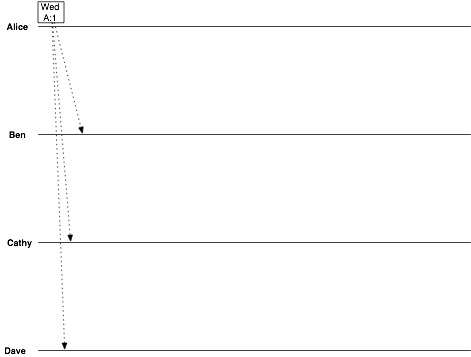
\includegraphics[width=\textwidth]{vector1}			
		\end{column}
		\begin{column}{0.5\textwidth}				
			\begin{lstlisting}[language=Python]
date = Wednesday
vclock = Alice:1
			\end{lstlisting}
		\end{column}	
	\end{columns} 
	\end{gdblank}
	\cprotEnv\begin{gdblank}
	\begin{columns}
		\begin{column}{0.5\textwidth}
			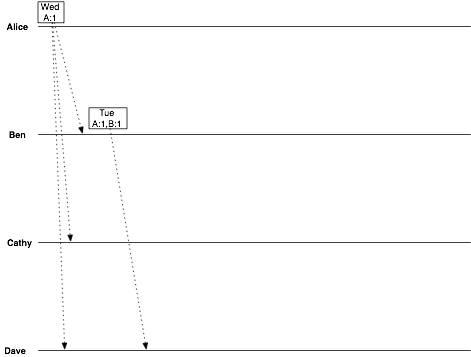
\includegraphics[width=\textwidth]{vector2}			
		\end{column}
		\begin{column}{0.5\textwidth}				
			Ben suggests Tuesday
			\begin{lstlisting}[language=Python]
date = Tuesday
vclock = Alice:1, Ben:1
			\end{lstlisting}
		\end{column}	
	\end{columns} 
	\end{gdblank}
	\cprotEnv\begin{gdblank}
	\begin{columns}
		\begin{column}{0.5\textwidth}
			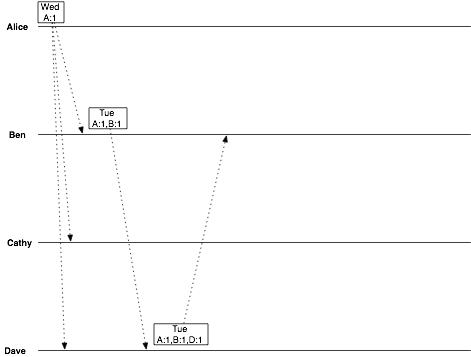
\includegraphics[width=\textwidth]{vector3}			
		\end{column}
		\begin{column}{0.5\textwidth}				
			Dave replies, confirming Tuesday
			\begin{lstlisting}[language=Python]
date = Tuesday
vclock = Alice:1, Ben:1, Dave:1
			\end{lstlisting}
		\end{column}	
	\end{columns} 
	\end{gdblank}
	\cprotEnv\begin{gdblank}
	\begin{columns}
		\begin{column}{0.5\textwidth}
			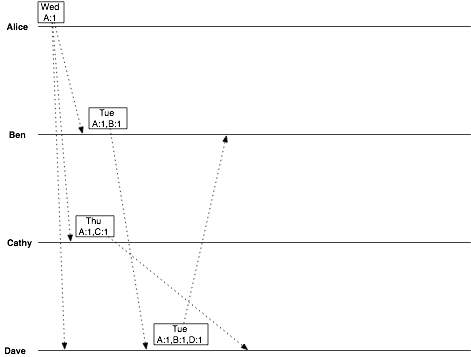
\includegraphics[width=\textwidth]{vector4}			
		\end{column}
		\begin{column}{0.5\textwidth}				
			Then Cathy joins, suggesting Thursday
			\begin{lstlisting}[language=Python]
date = Thursday
vclock = Alice:1, Cathy:1
			\end{lstlisting}
		\end{column}	
	\end{columns} 
	\end{gdblank}
	\cprotEnv\begin{gdblank}
	\begin{columns}
		\begin{column}{0.5\textwidth}
			\includegraphics[width=\textwidth]{vector4}			
		\end{column}
		\begin{column}{0.5\textwidth}				
			Dave has two conflicting objects
			\begin{lstlisting}[language=Python]
date = Tuesday
vclock = Alice:1, Ben:1, Dave:1
			\end{lstlisting}
			and
			\begin{lstlisting}[language=Python]
date = Thursday
vclock = Alice:1, Cathy:1
			\end{lstlisting}
		\end{column}	
	\end{columns} 
	\end{gdblank}
	\cprotEnv\begin{gdblank}
	\begin{columns}
		\begin{column}{0.5\textwidth}
			\includegraphics[width=\textwidth]{vector5}			
		\end{column}
		\begin{column}{0.5\textwidth}				
			Dave’s a reasonable guy, and chooses Thursday.\\So he sends this value back to Cathy
			\begin{lstlisting}[language=Python]
date = Thursday
vclock = Alice:1, Ben:1, Cathy:1, Dave:2
			\end{lstlisting}
		\end{column}	
	\end{columns} 
	\end{gdblank}
	\cprotEnv\begin{gdblank}
	\begin{columns}
		\begin{column}{0.5\textwidth}
			\includegraphics[width=\textwidth]{vector6}			
		\end{column}
		\begin{column}{0.5\textwidth}				
			When Alice asks Ben and Cathy for the latest decision, the replies she receives are, from Ben
			\begin{lstlisting}[language=Python]
date = Tuesday
vclock = Alice:1, Ben:1, Dave:1
			\end{lstlisting}
			From Cathy and Dave
			\begin{lstlisting}[language=Python]
date = Thursday
vclock = Alice:1, Ben:1, Cathy:1, Dave:2
			\end{lstlisting}
		\end{column}	
	\end{columns} 
	\end{gdblank}
	\cprotEnv\begin{gdblank}
	\begin{columns}
		\begin{column}{0.5\textwidth}
			\includegraphics[width=\textwidth]{vector7}			
		\end{column}
		\begin{column}{0.5\textwidth}				
			All Alice has to do is show Ben the vector clock from Cathy’s message, and Ben will know that he has been overruled.
		\end{column}	
	\end{columns} 
	\end{gdblank}
	\cprotEnv\begin{gdblank}
	\begin{columns}
		\begin{column}{0.5\textwidth}
			\includegraphics[width=\textwidth]{vector8}			
		\end{column}
		\begin{column}{0.5\textwidth}				
			Done. Everybody's in sync
		\end{column}	
	\end{columns} 
	\end{gdblank}
	\begin{gdblank}		
		\centering
		\includegraphics[height=\textheight]{mafia}
	\end{gdblank}
	\begin{gdblank}
		\frametitle{So, What!?}
		\centering
		\large 
		So... What Did We Get Out Of All of This?
	\end{gdblank}	
	% \begin{gdblank}
	% 	\frametitle{The WHY of things}
	% 	\begin{itemize}
	% 		\item The concept of causality between events is fundamental to the design and analysis of parallel and distributed computing and operating systems
	% 		\item Usually causality is tracked using physical time
	% 		      \pause 
	% 		      \item\bf\LARGE In distributed systems, it is not possible to have a global physical time
	% 	\end{itemize}		
	% \end{gdblank}

	\begin{gdblank}
		\frametitle{Review}
		\begin{itemize}
			\large
			\item Physical Clocks - hard to keep synchronized
			\item Logical clocks - can provide some notion of relative events occurrence
			\item Lamport's logical time
			      \begin{itemize}
			      	\item happened before defines causal relation
			      	\item this clocks don't capture causality
			      	\item total ordering relation
			      \end{itemize}
			\item Vector Clocks
			      \begin{itemize}
			      	\item captures causality
			      	\item have a component for each process in the system
			      	\item slow and grow
			      \end{itemize}
		\end{itemize}
	\end{gdblank} 
	\begin{gdblank}
		\frametitle{So many things to tell you}
		\begin{itemize}
			\item GPS Clocks
			\item Atomic Clocks in Google Spanner Database
			\item UTC, TAI, TCG and TCB coordinate time standards
			\item Why do clocks run clockwise?
			\item Why there were no December 30 in Samoa?
		\end{itemize}
	\end{gdblank} 
	\begin{gdblank}
		\frametitle{Thank you! That was Algebraic! Questions?}
		\begin{columns}
			\begin{column}{0.5\textwidth}
				\begin{itemize}
					\item Thank
					\item You 
					\item For
					\item Your
					\item Time
				\end{itemize}
				% Hope your software will never run on a space ship that is orbiting a black hole				
			\end{column}
			\begin{column}{0.5\textwidth}				
				\includegraphics[width=0.9\textwidth]{thankyou}			
			\end{column}	
		\end{columns} 		
	\end{gdblank} 	
\end{document}
% IT's hard but we could deal with it
% Java code


% https://literature.rockwellautomation.com/idc/groups/literature/documents/wp/enet-wp030_-en-e.pdf
% gps clocks

% There is no one simple definition of time. Time is something we deal with every day, and something that everyone thinks they understand.
% most people take for granted every day.
% What is the time?
% Time is a way to order a set of events? % Half life 3
% Einstein Space-Time
% We don't know exactly what the time is
% That's why religions as Zurvanizm apear
% But we take this as ordered
% Okey Falsehoods programmers believe about time
% There are always 24 hours in a day.
% Years have 365 days.
% Ok, that’s not true. But at least the time zone in which a program has to run will never change.
% The system clock will always be set to a time that is not wildly different from the correct local time.
% Time has no beginning and no end. Wiki The Year 2038 problem relates to representing time in many digital systems as the number of seconds passed since 1 January 1970 and storing it as a signed 32-bit binary integer.
% Time stamps will always have the same level of precision.
% A timestamp represents the time that an event actually occurred.
% Minute could be longer than an hour 
% The same month has the same number of days in it everywhere!
% Unix time is the number of seconds since Jan 1st 1970.
% You can wait for the clock to reach exactly HH:MM:SS by sampling once a second.
% The software will never run on a space ship that is orbiting a black hole.
% September 1752 had 19 days in British Empire
% doesn't a month always end in the same year it started? 

% Even JVM and Linux are bad
% Move to distributed system. What is simultanious
% Time-Space relativity
% Cake is lie
% Ok, what we have
% Physical Clocks
% With the timer we can define: simultaneous: all actions that happen between clock ticks before: an operation that happens in a previous clock tick after: an operation that happens in a subsequent clock tick
% Multiple systems - clock skew. On any two given computers, the drift rate will likely differ.
% To solve this problem, clock synchronization algorithms are necessary.
% Clocks sync overview
% Negative time correction?
% It is not important that all processes agree on what the actual time is, but that they agree on the order in which events occur.
% Lampard Clocks - The important contribution of Lamport is that in a distributed system, clocks need not be synchronized absolutely.
% Lampard Happens Before - Defines a relationship called “happens-before”. a -> b is read as “a happens before b” 
% That's how mafia works
% Vector Clocks
% We can use this capability to build a truly distributed dataflow graph with dependencies without having a centralized coordinating process.
% Cassandra


% The concept of causality between events is fundamental to the design and
% analysis of parallel and distributed computing and operating systems.
% Usually causality is tracked using physical time.
% In distributed systems, it is not possible to have a global physical time.
% As asynchronous distributed computations make progress in spurts, the
% logical time is sufficient to capture the fundamental monotonicity property
% associated with causality in distributed systems

% http://books.cs.luc.edu/distributedsystems/clocks.html#time-and-computation
% https://bugs.java.com/bugdatabase/view_bug.do?bug_id=6900441
% https://bbossola.wordpress.com/2013/09/04/jvm-issue-concurrency-is-affected-by-changing-the-date-of-the-system/
% http://yourcalendricalfallacyis.com/
% https://news.ycombinator.com/item?id=4128208
% https://infiniteundo.com/post/25326999628/falsehoods-programmers-believe-about-time#_=_
